\documentclass{article}

% TODO, for submission
% - Remove [preprint]
% - Remove title footnote
% - Add checklist
% - Remove vspace in Section 2 Heading

% if you need to pass options to natbib, use, e.g.:
%     \PassOptionsToPackage{numbers, compress}{natbib}
% before loading neurips_2024


% ready for submission
%\usepackage{neurips_2024}
%\usepackage[preprint]{neurips_2024}
\usepackage[final]{neurips_2024}

% to compile a preprint version, e.g., for submission to arXiv, add add the [preprint] option
% to compile a camera-ready version, add the [final] option
% to avoid loading the natbib package, add option nonatbib:
%    \usepackage[nonatbib]{neurips_2024}

\usepackage[utf8]{inputenc} % allow utf-8 input
\usepackage[T1]{fontenc}    % use 8-bit T1 fonts
\usepackage{hyperref}       % hyperlinks
\usepackage{url}            % simple URL typesetting
\usepackage{booktabs}       % professional-quality tables
\usepackage{amsfonts}       % blackboard math symbols
\usepackage{nicefrac}       % compact symbols for 1/2, etc.
\usepackage{microtype}      % microtypography
\usepackage{xcolor}         % colors

%%%%%%%%%%%%%%%%%%%%%%%%%%%%%%%%%%%%%
% WE ADD HERE ADDITIONAL PACKAGES
%%%%%%%%%%%%%%%%%%%%%%%%%%%%%%%%%%%%%
\usepackage{mathtools}
\usepackage{subcaption}
\usepackage{wrapfig}
\usepackage{cite}           % magical 
\usepackage[ruled, vlined]{algorithm2e}
\usepackage{sidecap}
\usepackage{array}
\sidecaptionvpos{figure}{c}
% Tikz
\usepackage{tikz}
\usetikzlibrary{arrows,arrows.meta,calc}
\usetikzlibrary{patterns,backgrounds}
\usetikzlibrary{positioning,fit}
\usetikzlibrary{shapes.geometric,shapes.multipart}
\usetikzlibrary{patterns.meta,decorations.pathreplacing,calligraphy}
\usetikzlibrary{tikzmark}
\usetikzlibrary{decorations.pathmorphing}

%%%%%%%%%%%%%%%%%%%%%%%%%%%%%%%%%%%%%
% COMMANDS
%%%%%%%%%%%%%%%%%%%%%%%%%%%%%%%%%%%%%
\newcommand{\x}{\mathbf{x}}
\newcommand{\z}{\mathbf{z}}
\newcommand{\y}{\mathbf{y}}
\newcommand{\w}{\mathbf{w}}
\newcommand{\bo}{\mathbf{o}}
\newcommand{\ba}{\mathbf{a}}
\newcommand{\bz}{\mathbf{z}}
\newcommand{\bs}{\mathbf{s}}
\newcommand{\scoref}{\nabla_\x \log p^\tau(\x)}
\newcommand{\scorem}{\mathbf{S}_\theta(\x, \tau)}
\newcommand{\bbe}{\mathbb{E}}
\newcommand{\Tau}{\mathcal{T}}

\newcommand{\repolink}{\href{https://github.com/eloialonso/diamond}{\texttt{https://github.com/eloialonso/diamond}}}
\newcommand{\wslink}{\href{https://diamond-wm.github.io}{\texttt{https://diamond-wm.github.io}}}
%\newcommand{\repolink}{\href{https://anonymous.4open.science/r/_diamond}{\textit{https://anonymous.4open.science/r/\_diamond}}}


\title{Diffusion for World Modeling:\\Visual Details Matter in Atari\thanks{To prevent confusion, this is the final version of \citep{alonso2023diffusion} and is not related to \citep{ding2024diffusion}.}}


% The \author macro works with any number of authors. There are two commands
% used to separate the names and addresses of multiple authors: \And and \AND.
%
% Using \And between authors leaves it to LaTeX to determine where to break the
% lines. Using \AND forces a line break at that point. So, if LaTeX puts 3 of 4
% authors names on the first line, and the last on the second line, try using
% \AND instead of \And before the third author name.

\author{%
  Eloi Alonso\thanks{Equal contribution. $^\ddagger$Equal supervision. Contact: \texttt{eloi.alonso@unige.ch} and \texttt{adam.jelley@ed.ac.uk}}\\
  University of Geneva
  \And
  Adam Jelley$^*$\\ 
  University of Edinburgh
  \And
  Vincent Micheli\\
  University of Geneva
  \And
  Anssi Kanervisto\\
  Microsoft Research
  \And
  Amos Storkey\\
  University of Edinburgh
  \And
  Tim Pearce$^\ddagger$\\\
  Microsoft Research
  \And
  Fran\c{c}ois Fleuret$^\ddagger$\\
  University of Geneva
}
% \author{%
%   David S.~Hippocampus\thanks{Use footnote for providing further information
%     about author (webpage, alternative address)---\emph{not} for acknowledging
%     funding agencies.} \\
%   Department of Computer Science\\
%   Cranberry-Lemon University\\
%   Pittsburgh, PA 15213 \\
%   \texttt{hippo@cs.cranberry-lemon.edu} \\
  % examples of more authors
  % \And
  % Coauthor \\
  % Affiliation \\
  % Address \\
  % \texttt{email} \\
  % \AND
  % Coauthor \\
  % Affiliation \\
  % Address \\
  % \texttt{email} \\
  % \And
  % Coauthor \\
  % Affiliation \\
  % Address \\
  % \texttt{email} \\
  % \And
  % Coauthor \\
  % Affiliation \\
  % Address \\
  % \texttt{email} \\
% }




\begin{document}


\maketitle


\begin{abstract}
Diffusion Models have emerged as powerful generative models for high-quality image synthesis, with many subsequent image editing techniques based on them. However, the ease of text-based image editing introduces significant risks, such as malicious editing for scams or intellectual property infringement. Previous works have attempted to safeguard images from diffusion-based editing by adding imperceptible perturbations. These methods are costly and specifically target prevalent Latent Diffusion Models (LDMs), while Pixel-domain Diffusion Models (PDMs) remain largely unexplored and robust against such attacks. Our work addresses this gap by proposing a novel attacking framework with a feature representation attack loss that exploits vulnerabilities in denoising UNets and a latent optimization strategy to enhance the naturalness of protected images. Extensive experiments demonstrate the effectiveness of our approach in attacking dominant PDM-based editing methods (e.g., SDEdit) while maintaining reasonable protection fidelity and robustness against common defense methods. Additionally, our framework is extensible to LDMs, achieving comparable performance to existing approaches.
\end{abstract}

\section{Introduction}
%
Large Transformers have enabled a number of breakthrough advances in modeling language, vision, audio, biology and numerous other domains \citep{vaswani2017attention}, \citep{dosovitskiy2020image}, \citep{radford2022robust}, \citep{cramer2021alphafold2}. Much of the success of Transformers, powered by the attention operator \citep{vaswani2017attention}, relies on their scaling properties \citep{hoffmann2022training} and the emergence of in-context learning \citep{garg2022can}, which allows them to generalize to unseen data and tasks given context as input. 
%
The Transformer block is a powerful tool for sequence modeling, but it is not without its limitations. One of the most notable is the computational cost, which grows rapidly as the length of the input sequence increases. Specifically, the cost scales quadratically with the length $L$ of the sequence, which places a strict limit on the amount of context that can be considered by the model.
%
Breaking the quadratic barrier is a key step towards new possibilities for deep learning, such as using entire textbooks as context, generating long-form music or processing gigapixel scale images.

Efforts to reduce the computational cost of attention in models primarily involve the use of linearized, low-rank, and sparse approximations \citep{child2019generating,wang2020linformer,kitaev2020reformer,zhai2021attention,roy2021efficient,schlag2021linear,tu2022maxvit}. These approaches introduce a trade-off between expressivity and speed, requiring hybridization with standard attention layers to reach Transformer quality \citep{mehta2022long,dao2022hungry}.

A growing amount of evidence suggests that attention mechanisms only utilize a small portion of their quadratic capabilities for language processing \citep{olsson2022context, dao2022hungry}, leading us to question its role as the gold-standard operator for deep learning at scale. Specifically, we ask:

%
\begin{figure*}[t]
    \centering
    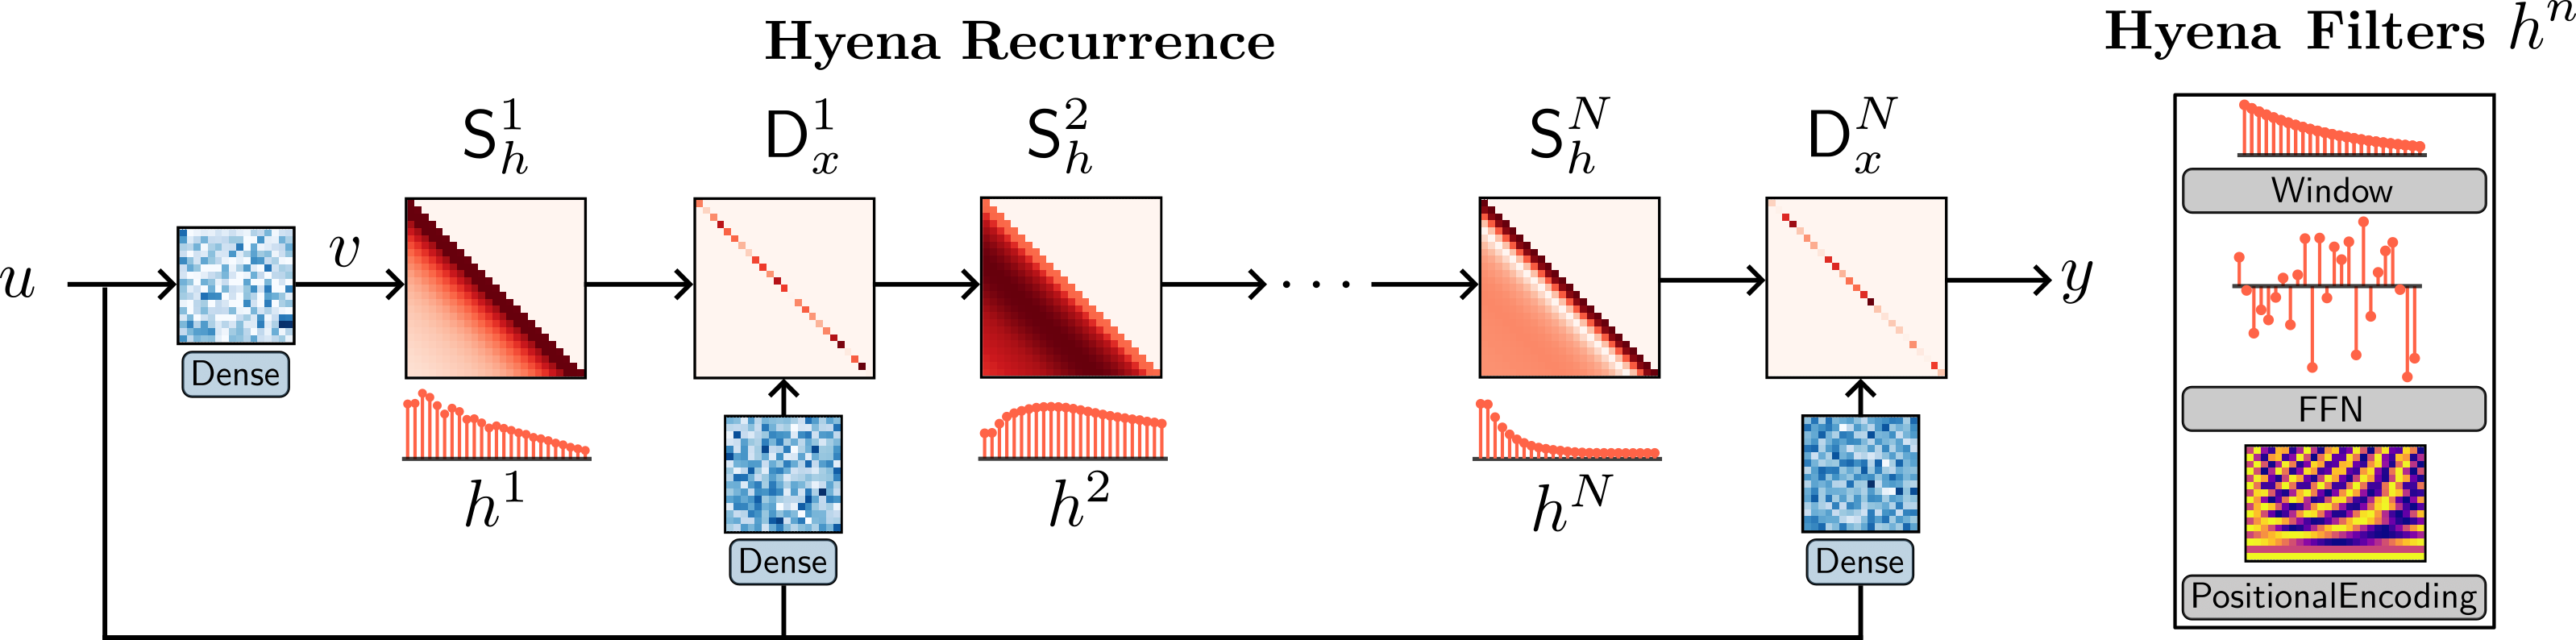
\includegraphics[width=\linewidth]{figures/hyena.png}
    \vspace{-2mm}
    \caption{The ${\sf Hyena}$ operator is defined as a recurrence of two efficient subquadratic primitives: an implicit long convolution $h$ (i.e. {\sf Hyena} filters parameterized by a feed-forward network) and multiplicative element-wise gating of the (projected) input. The depth of the recurrence specifies the size of the operator. {\sf Hyena} can equivalently be expressed as a multiplication with \textit{data-controlled} (conditioned by the input $u$) diagonal matrices $\sD_x$ and Toeplitz matrices $\sS_h$. In addition, {\sf Hyena} exhibits sublinear parameter scaling (in sequence length) and unrestricted context, similar to attention, while having lower time complexity.}
    \label{arch}
\end{figure*}
%

{\centering
\textit{Are there subquadratic operators that can match the quality of attention at scale?}\par}

\vspace{0.5cm}
% 

We obtain a positive answer based on a composition of efficient subquadratic primitives, such as \textit{element-wise multiplication} (gating) and \textit{long convolutions} i.e., convolutions with filter sizes as long as the input. We rely on a set of targeted reasoning tasks, grounded in recent work on \textit{mechanistic interpretability} \citep{elhage2021mathematical,power2022grokking,olsson2022context,zhang2022unveiling} such as recall and induction, to distill three properties of attention correlated with its performance and the quality gap with existing subquadratic approaches: 
%
\begin{itemize}[leftmargin=0.1in]
    \item[$a.$] \textbf{Data control:} Attention implements an expressive \textit{data-controlled} \citep{massaroli2020dissecting} linear operator\footnote{Self-attention can be expressed as $y = \sA(k, q) v$ where $\sA$ is the \textit{attention matrix} conditioned by linear projections $k, q$ of the input and multiplied by $v$, another projection.}, encoding an entire family of linear functions in a single block.
    \item[$b.$] \textbf{Sublinear parameter scaling:} Parameter counts of attention layers are decoupled from sequence length, allowing Transformers to allocate more parameters elsewhere e.g., the \textit{feed-forward neural networks} ({$\sf FFN$s}) between attention layers.
    \item[$c.$] \textbf{Unrestricted context:} For a given input, attention has an unrestricted context i.e., it can approximate dependencies between any two inputs, without arbitrary restrictions such as locality (except in cases using masking such as autoregressive models).
\end{itemize}
%
\paragraph{The ${\sf Hyena}$ hierarchy}
%
Guided by these findings, we introduce the ${\sf Hyena}$ hierarchy, an operator defined by a recurrence of two efficient subquadratic primitives: \textbf{a long convolution and element-wise multiplicative gating} (see Figure \ref{arch}). A specified depth (i.e., number of steps) of the recurrence controls the size of the operator. For short recurrences, existing models are recovered as special cases \citep{mehta2022long,dao2022hungry}. By mapping each step in the ${\sf Hyena}$ recurrence to its corresponding matrix form, we reveal ${\sf Hyena}$ operators to be equivalently defined as a decomposition of a \textit{data-controlled} matrix i.e., a matrix whose entries are functions of the input. Furthermore, we show how ${\sf Hyena}$ operators can be evaluated efficiently without materializing the full matrix, by leveraging fast convolution algorithms \citep{selesnick2017fast}. Empirically, ${\sf Hyena}$ operators are able to significantly shrink the quality gap with attention at scale, reaching similar perplexity and downstream performance with a smaller computational budget (Section \ref{res:lm}) and \textbf{without hybridization} of attention.
%

\paragraph{Narrowing the capabilities gap}
%
The design of {\sf Hyena} is motivated by a quality gap between standard dense attention and alternative subquadratic operators, which we identify by focusing on reasoning tasks correlated with language modeling performance at scale. We extend the suite of basic mechanistic interpretability benchmarks (\textit{induction} and \textit{recall}) with additional tasks that probe how quickly model performance degrades when task complexity increases (e.g. vocabulary size grows). In addition, we investigate the optimal parameterization of long convolutions in ${\sf Hyena}$. In the most challenging settings with hundreds of thousands of tokens, our implicit parameterization scheme improves over other operators leveraging state spaces \citep{gu2021efficiently}, frequency-domain parametrizations \citep{li2020fourier}, or standard convolutions by over $50\%$ accuracy.
%
\paragraph{Scaling in language and vision}
%
Next, we aim to verify whether rankings in our reasoning benchmark suite are predictive of quality at scale. We test ${\sf Hyena}$ on autoregressive language modeling at the sub-billion parameter scale, setting a new state-of-the-art for dense-attention-free architectures in standard datasets ({\sc WikiText103} and {\sc The Pile}) and matching Transformer quality. On the {\sc The Pile} at the $335$M parameter scale, we match Transformer perplexity with a $20\%$ reduction in the total count of \textit{floating point operations} (FLOPs). As an extension, we investigate the generality of ${\sf Hyena}$ operators by testing on large-scale image recognition, replacing attention in the Vision Transformer (ViT) \citep{dosovitskiy2020image}. In image classification, ${\sf Hyena}$ is able to match attention in accuracy when training on ImageNet-1k from scratch.
%
\paragraph{Toward much longer context}
%
Finally, we benchmark the efficiency of ${\sf Hyena}$ on long sequences. We measure $5$x speedups over dense self-attention at length $8192$ -- $2$x over highly optimized FlashAttention\footnote{FlashAttention is already 2-4x faster than a standard attention implementation in PyTorch.} \citep{dao2022flashattention} -- and $100$x speedup over FlashAttention at sequence lengths of $64$k, where standard attention implementation in PyTorch runs out of memory. 
\vspace{-0.1cm}
\section{Preliminaries}
\label{sec:framework}
\vspace{-0.1cm}

\subsection{Reinforcement learning and world models}
\label{subsec:pomdp_and_wm}

We model the environment as a standard Partially Observable Markov Decision Process (\textsc{pomdp}) \citep{sutton2018reinforcement}, $(\mathcal{S}, \mathcal{A}, \mathcal{O},T,R,O,\gamma)$, where $\mathcal{S}$ is a set of states, $\mathcal{A}$ is a set of discrete actions, and $\mathcal{O}$ is a set of image observations. The transition function $T: \mathcal{S} \times \mathcal{A} \times \mathcal{S} \to [0,1]$ describes the environment dynamics $p(\mathbf{s}_{t+1} \mid \mathbf{s}_t, \ba_t)$, and the reward function $R: \mathcal{S} \times \mathcal{A} \times \mathcal{S} \to \mathbb{R}$ maps transitions to scalar rewards. Agents cannot directly access states $s_t$ and only see the environment through image observations $x_t \in \mathcal{O}$, emitted according to observation probabilities $p(\x_t \mid \mathbf{s}_t)$, described by the observation function $O: \mathcal{S} \times \mathcal{O} \to [0,1]$. The goal is to obtain a policy $\pi$ that maps observations to actions in order to maximize the expected discounted return $\mathbb{E}_\pi[\sum_{t \ge 0} \gamma^t r_t]$, where $\gamma \in [0,1]$ is a discount factor. World models \citep{ha2018world} are generative models of environments, i.e. models of $p(s_{t+1},r_{t} \mid s_t, a_t)$. These models can be used as simulated environments to train RL agents \citep{sutton1991dyna} in a sample-efficient manner \citep{wu2023daydreamer}. In this paradigm, the training procedure typically consists of cycling through the three following steps: collect data with the RL agent in the real environment; train the world model on all the collected data; train the RL agent in the world model environment (commonly referred to as "in imagination"). 

\subsection{Score-based diffusion models}
\label{subsec:diffusion}

Diffusion models \citep{sohl2015difforigin} are a class of generative models inspired by non-equilibrium thermodynamics that generate samples by reversing a noising process.

We consider a diffusion process $\{\x^\tau\}_{\tau \in [0,\Tau]}$ indexed by a continuous time variable $\tau \in [0,\Tau]$, with corresponding marginals $\{p^\tau\}_{\tau \in [0,\Tau]}$, and boundary conditions $p^0 = p^{data}$ and $p^\Tau = p^{prior}$, where $p^{prior}$ is a tractable unstructured prior distribution, such as a Gaussian. Note that we use $\tau$ and superscript for the diffusion process time, in order to keep $t$ and subscript for the environment time.

This diffusion process can be described as the solution to a standard stochastic differential equation (SDE) \citep{song_sde},
\begin{equation}
\label{eq:forward_process}
    d\x = \mathbf{f} (\x, \tau) d\tau +  g(\tau) d\w, 
\end{equation}
where $\w$ is the Wiener process (Brownian motion), $\mathbf{f}$ a vector-valued function acting as a drift coefficient, and  $g$ a scalar-valued function known as the diffusion coefficient of the process.

To obtain a generative model, which maps from noise to data, we must reverse this process. Remarkably, \citet{anderson1982reverse} shows that the reverse process is also a diffusion process, running backwards in time, and described by the following SDE,
\begin{equation}
\label{eq:reverse_process}
    d\x = [\mathbf{f} (\x, \tau) - g(\tau)^2 \scoref] d\tau +  g(\tau) d\Bar{\w}, 
\end{equation}
where $\Bar{\w}$ is the reverse-time Wiener process, and $\scoref$ is the (Stein) score function, the gradient of the log-marginals with respect to the support. Therefore, to reverse the forward noising process, we are left to define the functions $f$ and $g$ (in Section \ref{subsec:practical_dwm}), and to estimate the unknown score functions $\scoref$, associated with marginals $\{p^\tau\}_{\tau \in [0,\Tau]}$ along the process. In practice, it is possible to use a single time-dependent score model $\scorem$ to estimate these score functions \citep{song_sde}.

At any point in time, estimating the score function is not trivial since we do not have access to the true score function. Fortunately, \citet{hyvarinen2005estimation} introduces the \textit{score matching} objective, which surprisingly enables training a score model from data samples without the knowledge of the underlying score function. To access samples from the marginal $p^\tau$, we need to simulate the forward process from time $0$ to time $\tau$, as we only have clean data samples. This is costly in general, but if $f$ is affine, we can analytically reach any time $\tau$ in the forward process in a single step, by applying a Gaussian perturbation kernel $p^{0\tau}$ to clean data samples \citep{song_sde}. Since the kernel is differentiable, score matching simplifies to a \textit{denoising score matching} objective \citep{vincent2011connection},

\begin{equation}
\label{eq:denoising_sm}
    \mathcal{L}(\theta) = \bbe \left[ \Vert \mathbf{S}_\theta(\x^\tau, \tau) - \nabla_{\x^\tau} \log p^{0\tau}(\x^\tau \mid \x^0) \Vert^2 \right],
\end{equation}

where the expectation is over diffusion time $\tau$, noised sample $\x^\tau \sim p^{0\tau}(\x^\tau \mid \x^0)$, obtained by applying the $\tau$-level perturbation kernel to a clean sample $\x^0 \sim p^{data}(\x^0)$. Importantly, as the kernel $p^{0\tau}$ is a known Gaussian distribution, this objective becomes a simple $L_2$ reconstruction loss,

\begin{equation}
\label{eq:reconstruction_sm}
     \mathcal{L}(\theta) = \bbe \left[ \Vert \mathbf{D}_\theta(\x^\tau, \tau) - \x^{0} \Vert^2 \right],
\end{equation}

with reparameterization $\mathbf{D}_\theta(\x^\tau, \tau) = \mathbf{S}_\theta(\x^\tau, \tau) \sigma^2(\tau) + \x^\tau$, where $\sigma(\tau)$ is the variance of the $\tau$-level perturbation kernel.



\subsection{Diffusion for world modeling}
\label{subsec:dwm_training}

%The score-based diffusion model described in Section \ref{subsec:diffusion} provides an unconditional generative model of $p_{data}$. To serve as a world model, we need a conditional generative model of the environment dynamics, $p(s_{t+1} \mid s_t, a_t)$. Since we consider the more general case of a \textsc{pomdp} where the Markovian state is unknown, we instead approximate this state with a buffer of recent observations and actions. We condition a diffusion model  with this buffer, to estimate $p(\x_{t+1} \mid \x_{\le t}, a_{\le t})$ and generate the next observation directly, as demonstrated in Figure \ref{fig:architecture}. This modifies Equation \ref{eq:reconstruction_sm} as follows,

The score-based diffusion model described in Section \ref{subsec:diffusion} provides an unconditional generative model of $p_{data}$. To serve as a world model, we need a conditional generative model of the environment dynamics, $p(\x_{t+1} \mid \x_{\le t}, a_{\le t})$, where we consider the general case of a \textsc{pomdp}, in which the Markovian state $s_t$ is unknown and can be approximated from past observations and actions. We can condition a diffusion model on this history, to estimate and generate the next observation directly, as shown in Figure \ref{fig:architecture}. This modifies Equation \ref{eq:reconstruction_sm} as follows,
\begin{equation}
\label{eq:denoising_sm_conditional}
     \mathcal{L}(\theta) = \bbe \left[ \Vert \mathbf{D}_\theta(\x_{t+1}^\tau, \tau, \x_{\le t}^0, a_{\le t}) - \x_{t+1}^0 \Vert^2 \right].
\end{equation}
\vspace{-5mm}

During training, we sample a trajectory segment $\x_{\le t}^0, a_{\le t}, \x_{t+1}^0$ from the agent's replay dataset, and we obtain the noised next observation $\x_{t+1}^\tau \sim p^{0\tau}(\x_{t+1}^\tau \mid \x_{t+1}^0)$ by applying the $\tau$-level perturbation kernel. In summary, this diffusion process for world modeling resembles the standard diffusion process described in Section \ref{subsec:diffusion}, with a score model conditioned on past observations and actions.

To sample the next observation, we iteratively solve the reverse SDE in Equation \ref{eq:reverse_process}, as illustrated in Figure \ref{fig:architecture}. While we can in principle resort to any ODE or SDE solver, there is an inherent trade-off between sampling quality and Number of Function Evaluations (NFE), that directly determines the inference cost of the diffusion world model (see Appendix \ref{appendix:sampling} for more details).

\section{Method}
\label{sec:method}

\subsection{Practical choice of diffusion paradigm}
\label{subsec:practical_dwm}

Building on the background provided in Section \ref{sec:framework}, we now introduce \textsc{diamond} as a practical realization of a diffusion-based world model. In particular, we now define the drift and diffusion coefficients $\mathbf{f}$ and $g$ introduced in Section \ref{subsec:diffusion}, corresponding to a particular choice of diffusion paradigm. While \textsc{ddpm} \citep{ho2020DDPM} is an example of one such choice (as described in Appendix \ref{app:ddpm}) and would historically be the natural candidate, we instead build upon the \textsc{edm} formulation proposed in \citet{karras2022elucidating}. The practical implications of this choice are discussed in Section \ref{subsec:diffusion_choice}. In what follows, we describe how we adapt \textsc{edm} to build our diffusion-based world model.

We consider the perturbation kernel $p^{0\tau}(\x_{t+1}^\tau \mid \x_{t+1}^0) = \mathcal{N}(\x_{t+1}^\tau; \x_{t+1}^0, \sigma^2(\tau) \mathbf{I})$, where $\sigma(\tau)$ is a real-valued function of diffusion time called the noise schedule. This corresponds to setting the drift and diffusion coefficients to $\mathbf{f}(\x, \tau) = \mathbf{0}$ (affine) and $g(\tau) = \sqrt{2 \dot \sigma(\tau) \sigma(\tau)}$.

We use the network preconditioning introduced by \citet{karras2022elucidating} and so parameterize $\mathbf{D}_\theta$ in Equation \ref{eq:denoising_sm_conditional} as the weighted sum of the noised observation and the prediction of a neural network $\mathbf{F}_\theta$,
\begin{equation}
\label{eq:karras_wrappers} 
    \mathbf{D}_\theta(\x_{t+1}^\tau, y_t^\tau) = c_\text{skip}^\tau \; \x_{t+1}^\tau + c_\text{out}^\tau \; \mathbf{F}_\theta \big( c_\text{in}^\tau \; \x_{t+1}^\tau, y_t^\tau \big),
\end{equation}
where for brevity we define $y_t^\tau \coloneqq (c_\text{noise}^\tau, \x^0_{\le t}, a_{\le t})$ to include all conditioning variables.

The preconditioners $c_\text{in}^\tau$ and $c_\text{out}^\tau$ are selected to keep the network's input and output at unit variance for any noise level $\sigma(\tau)$, $c_\text{noise}^\tau$ is an empirical transformation of the noise level, and $c_\text{skip}^\tau$ is given in terms of $\sigma(\tau)$ and the standard deviation of the data distribution $\sigma_\text{data}$, as $c_{skip}^\tau = \sigma_{data}^2/(\sigma_{data}^2 + \sigma^2(\tau))$. These preconditioners are fully described in Appendix \ref{appendix:karras_conditioners}.

Combining Equations \ref{eq:denoising_sm_conditional} and \ref{eq:karras_wrappers} provides insight into the training objective of $\mathbf{F}_\theta$,
\begin{align}
\label{eq:effective_obj}
\mathcal{L}(\theta)  = \bbe \Big[ \Vert 
\underbrace{\mathbf{F}_\theta \big( c_\text{in}^\tau \x_{t+1}^\tau, y_t^\tau \big)}_\text{Network prediction} - 
\underbrace{\frac{1}{c_\text{out}^\tau} \big( \x_{t+1}^0 - c_\text{skip}^\tau \x_{t+1}^\tau\big)}_\text{Network training target}
\Vert^2 \Big].
\end{align}
The network training target adaptively mixes signal and noise depending on the degradation level $\sigma(\tau)$.
When $\sigma(\tau) \gg \sigma_\text{data}$, we have $c_\text{skip}^\tau \to 0$, and the training target for $\mathbf{F}_\theta$ is dominated by the clean signal $\x_{t+1}^0$. Conversely, when the noise level is low, $\sigma(\tau) \to 0$, we have $c_\text{skip}^\tau \to 1$, and the target becomes the difference between the clean and the perturbed signal, i.e. the added Gaussian noise. Intuitively, this prevents the training objective to become trivial in the low-noise regime. In practice, this objective is high variance at the extremes of the noise schedule, so \citet{karras2022elucidating} sample the noise level $\sigma(\tau)$ from an empirically chosen log-normal distribution in order to concentrate the training around medium-noise regions, as described in Appendix \ref{appendix:karras_conditioners}.

We use a standard U-Net 2D for the vector field $\mathbf{F}_\theta$ \citep{ronneberger2015unet}, and we keep a buffer of $L$ past observations and actions that we use to condition the model. We concatenate these past observations to the next noisy observation channel-wise, and we input actions through adaptive group normalization layers \citep{adagn} in the residual blocks \citep{He2015} of the U-Net.

As discussed in Section \ref{subsec:dwm_training} and Appendix \ref{appendix:sampling}, there are many possible sampling methods to generate the next observation from the trained diffusion model. While our codebase supports a variety of sampling schemes, we found Euler's method to be effective without incurring the cost of additional NFE required by higher order samplers, or the unnecessary complexity of stochastic sampling.

\subsection{Reinforcement learning in imagination}
\label{subsec:rl}

Given the diffusion model from Section \ref{subsec:practical_dwm}, we now complete our world model with a reward and termination model, required for training an RL agent in imagination. Since estimating the reward and termination are scalar prediction problems, we use a separate model $R_\psi$ consisting of standard \textsc{cnn} \citep{cnn_lecun,He2015} and \textsc{lstm} \citep{lstm,Gers2000} layers to handle partial observability. The RL agent involves an actor-critic network parameterized by a shared \textsc{cnn-lstm} with policy and value heads. The policy $\pi_\phi$ is trained with \textsc{reinforce} with a value baseline, and we use a Bellman error with $\lambda$-returns to train the value network $V_\phi$, similar to \citet{iris2023}. We train the agent entirely in imagination as described in Section \ref{subsec:pomdp_and_wm}. The agent only interacts with the real environment for data collection. After each collection stage, the current world model is updated by training on all data collected so far. Then, the agent is trained with RL in the updated world model environment, and these steps are repeated. This procedure is detailed in Algorithm \ref{alg:diamond}, and is similar to \citet{kaiser2019atari100k,hafner2020dream,iris2023}. We provide architecture details, hyperparameters, and RL objectives in Appendices \ref{app:architectures}, \ref{app:hyperparams}, \ref{appendix:rl_actor_critic}, respectively.

\section{Experiments}
\subsection{Experimental Setting}
\noindent \textbf{Pretraining.} The SA-1B dataset  consists of 11M diverse, high resolution images with 1.1B high-quality segmentation masks. Similar to~\citep{ravi2024sam}, we pretrain our EfficientTAM without memory components on SA-1B dataset~\citep{kirillov2023segment} for 90k steps. Our ViT image encoder is initialized from pre-trained ViTs~\citep{xiong2024efficientsam}
. We use the AdamW optimizer ~\citep{loshchilov2017decoupled} with a momentum, ($\beta_1 = 0.9$, $\beta_2 = 0.999$), a global batch size of 256, and a initial learning rate of $4e-4$. The learning rate is decayed by a reciprocal square root learning rate schedule~\citep{zhai2022scaling} with 1k iterations linear warmup and 5k iterations linear cooldown. We set weight decay to 0.1. We do not apply drop path for our image encoder. Layer-wise decay~\citep{clark2020electra} is set to 0.8. We apply horizontal flip augmentation and resize the input image resolution to $1024\times 1024$. We restrict our training to $64$ masks per image. Our models are pre-trained on 256 A100 GPUs with 80GB GPU memory with a linear combination of focal and dice loss for mask prediction (e.g., a ratio of 20:1). Bfloat16 is used during the training.

\noindent \textbf{Full Training Datasets.} Following~\citep{ravi2024sam}, we train our EfficientTAM including memory components on SA-V dataset~\citep{ravi2024sam} and a 10\% subset of SA-1B~\citep{kirillov2023segment}. SA-V is a large-scale and diverse video segmentation dataset, including 51K videos captured across 47 countries and 600K mask annotations covering whole objects and parts. SA-V video resolution ranges from 240p to 4K and duration ranges from 4 seconds to 138 seconds. Unlike SAM 2, we do not use other open-source datasets or internal datasets during our training for a fair comparison with baselines. 

\noindent \textbf{Full Training Implementation Details.} Similar to  ~\citep{ravi2024sam}, we train our EfficientTAM for 300k steps after pretraining. We use the AdamW optimizer ~\citep{loshchilov2017decoupled} with a momentum, ($\beta_1 = 0.9$, $\beta_2 = 0.999$), a batch size of 256, and a initial learning rate of $6e-5$ for image encoder and $3e-4$ for other components of the model. The learning rate is decayed by a cosine schedule with 15k iterations linear warmup. We set weight decay to 0.1. We do not apply drop path for our image encoder. Layer-wise decay~\citep{clark2020electra} is set to 0.8. We apply horizontal flip image augmentation and resize the input image resolution to $1024\times 1024$. For video, we apply horizontal flip augmentation, affine transformation with degree $25$ and shear $20$, color jittering with brightness $0.1$, contrast $0.03$, saturation $0.03$, gray scale augmentation with a probability of $0.05$, We restrict our training to $64$ masks per image and $3$ masks per frame for video. Our models are trained on 256 A100-80G GPUs with a linear combination of focal and dice losses for mask prediction, mean-absolution-error loss for IoU prediction, and cross-entropy loss for object prediction. The ratio for the linear combination loss is 20:1:1:1. Bfloat16 is used for training.

\noindent \textbf{Downstream Tasks/Datasets/Models.} \underline{\textit{Tasks and Datasets.}} We consider zero-shot video tasks including promptable video segmentation and semi-supervised video object segmentation, and zero-shot image tasks to demonstrate the competing capabilities of EfficientTAM on image and video segmentation.
For zero-shot image tasks, we evaluate EfficientTAM on 37 datasets including 23 datasets of SA-23~\citep{kirillov2023segment} and 14 video datasets introduced in~\citep{ravi2024sam}. For zero-shot video tasks, we evaluate our EfficientTAM on 9 densely annotated datasets for promptable video segmentation. We use 17 video datasets to evaluate zero-shot accuracy under interactive semi-supervised VOS setting using different prompts. For the standard semi-supervised VOS setting where a ground-truth mask on the first frame is provided, MOSE~\citep{ding2023mose}, DAVIS2017~\citep{pont20172017}, LVOS~\citep{hong2024lvos}, SA-V~\citep{ravi2024sam}, and YTVOS~\citep{xu2018youtube} are used to measure the VOS accuracy. We refer readers to~\citep{kirillov2023segment,ravi2024sam} for the details of these datasets.
\underline{\textit{Models.}} We use our EfficientTAM for zero-shot image and video tasks.

\noindent\textbf{Baselines and Evaluation Metrics.}
\underline{\textit{Baselines.}} For the standard semi-supervised VOS task, where the first-frame mask is provided, we compare the performance of our EfficientTAM with SAM 2\citep{ravi2024sam}, Cutie-base\citep{cheng2024putting}, DEVA~\citep{cheng2023tracking}, XMem~\citep{cheng2022xmem}, etc.
For the zero-shot promptable video segmentation task and the interactive semi-supervised video object segmentation task using different prompts, we compare our method with SAM2~\citep{ravi2024sam}, SAM+XMem++~\citep{ravi2024sam}, and SAM+Cutie~\citep{ravi2024sam}. For zero-shot image segmentation task, we compare with SAM~\citep{kirillov2023segment} and SAM2~\citep{ravi2024sam}. Note that we use the opensource version of SAM 2 (without training on MOSE/LVOS/YTVOS) for comparison. We also acknowledge the very recent release of SAM 2.1 trained with long memory contexts. 
\underline{\textit{Evaluation Metrics.}} We evaluate our method and all baselines using the accuracy metrics of the combined $\mathcal{J}$(region similarity)\&$\mathcal{F}$(contour accuracy),  for zero-shot video segmentation tasks; mIoU (mean intersection over union) for zero-shot image segmentation tasks. For efficiency metrics, we compare the number of model parameters or inference throughput on GPU (e.g, A100) and latency on mobile devices (e.g., iPhone 15 Pro Max). We follow SAM 2~\citep{ravi2024sam} to report metrics. When providing main results on MOSE, LVOS and YTVOS, we submit to their benchmarking servers to evaluate on, \textit{MOSE val}, \textit{LVOS val}, and \textit{YTVOS2019 val}, for final performance. For ablation studies, we evaluate on a MOSE development set, \textit{MOSE dev} with 200 randomly-sampled videos from the MOSE training split~\citep{ravi2024sam}.

\subsection{Main Results}
% Please add the following required packages to your document preamble:
% \usepackage{multirow}
% Please add the following required packages to your document preamble:
% \usepackage{multirow}
\begin{table*}[t]
% \vspace{-3mm}
\centering
\resizebox{0.9\linewidth}{!}{
\begin{tabular}{c|cccc|c|c|c|c}
\hline
\multirow{2}{*}{Method}                                   & \multicolumn{4}{c|}{$\mathcal{J}$\&$\mathcal{F}$}                                                                                                                                                         & $\mathcal{G}$                                            & \multirow{2}{*}{\begin{tabular}[c]{@{}c@{}}\\Parameters\\ (M)\end{tabular}} & FPS   & Latency (ms) \\ \cline{2-6} \cline{8-9} 
                                                          & \begin{tabular}[c]{@{}c@{}}MOSE \\ val\end{tabular} & \begin{tabular}[c]{@{}c@{}}DAVIS\\ 2017 val\end{tabular} & \begin{tabular}[c]{@{}c@{}}LVOS\\ val\end{tabular} & \begin{tabular}[c]{@{}c@{}}SA-V\\ test\end{tabular} & \begin{tabular}[c]{@{}c@{}}YTVOS\\ 2019 val\end{tabular} &                                                                           & A100  & iPhone15     \\ \hline
STCN~\citep{cheng2021rethinking}                                                      & 52.5                                                & 85.4                                                     & -                                                  & 57.3                                                & 82.7                                                     &   54                                                                        & 62.8  & -            \\
% R50-AOT-L~\citep{yang2021associating}                                                 & 58.4                                                & 84.9                                                     & -                                                  & 56.7                                                & 85.3                                                     & 15                                                                          & 6.4   & -            \\
% DeAOT-R50~\citep{yang2022decoupling}                                                 & 64.1                                                & 86.0                                                     & -                                                  & 59.9                                                & 85.3                                                     &                                                              20             & 11.7  & -            \\
RDE~\citep{li2022recurrent}                                                       & 46.8                                                & 84.2                                                     & -                                                  & 48.4                                                & 81.9                                                     &      64                                                                     & 88.8  & -            \\
XMem~\citep{cheng2022xmem}                                                      & 59.6                                                & 86.0                                                     & -                                                  & 60.1                                                & 85.6                                                     &     62                                                                      & 61.2  & -            \\
% SimVOS-B~\citep{wu2023scalable}                                                 & -                                                   & 88.0                                                     & -                                                  & 41.2                                                & 84.2                                                     &                                                                           & 3.3   & -            \\
% JointFormer~\citep{zhang2023joint}                                               & -                                                   & 90.1                                                     & -                                                  & -                                                   & 87.4                                                     &                                                                           & 3.0   & -            \\
% ISVOS~\citep{wang2023look}                                                     & -                                                   & 88.2                                                     & -                                                  & -                                                   & 86.3                                                     &                                                                           & 5.8   & -            \\
DEVA~\citep{cheng2023tracking}                                                      & 66.0                                                & 87.0                                                     & 55.9                                               & 53.8                                                & 85.4                                                     &      69                                                                     & 65.2  & -            \\
Cutie-base~\citep{cheng2024putting}                                                & 69.9                                                & 87.9                                                     & 66.0                                               & 61.6                                                & 87.0                                                     & 35                                                                        & 65    & -            \\
Cutie-base+~\citep{cheng2024putting}                                               & 71.7                                                & 88.1                                                     & -                                                  & 62.3                                                & 87.5                                                     & 35                                                                        & 57.2  & -            \\
SAM 2~\citep{ravi2024sam}                                                     & 72.8                                                & 88.9                                                     &             76.2                                       &         74.7                                        & 87.9                                                     & 81                                                                        & 43.8  & -            \\ \hline
\rowcolor{gray} EfficientTAM-Ti/2 (ours) & 68.4                                                & 88.4                                                     & 66.1                                               & 70.8                                                & 87.1                                                     & 18                                                                        & 109.4 & 261.4        \\
\rowcolor{gray} EfficientTAM-Ti (ours)   & 69.3                                                & 89.1                                                     & 69.6                                               & 70.7                                                & 86.7                                                     & 18                                                                        & 96.2  & 840.5        \\
\rowcolor{gray} EfficientTAM-S/2 (ours)  & 70.8                                                & 88.6                                                     & 72.1                                               & 74.0                                                & 87.2                                                     & 34                                                                        & 109.4 & 450          \\
\rowcolor{gray} EfficientTAM-S (ours)    & 71.4                                                & 89.2                                                     & 73.4                                               & 74.5                                                & 87.2                                                     & 34                                                                        & 85.0  & 1010.8       \\ \hline
\end{tabular}}
\caption{Standard semi-supervised video object segmentation results across video object segmentation benchmarks.}
\label{tab:vos}
\end{table*}
\textbf{Standard Semi-Supervised Video Object Segmentation.} Semi-supervised video object segmentation is the process of object segmentation and tracking in a video based on a ground-truth mask on the first frame. We follow SAM 2~\citep{ravi2024sam} and report accuracy of our methods on this standard semi-supervised video object segmentation task. We also report latency on a single A100 GPU with a batch size of 1. We evaluate EfficientTAMs with different image encoders, ViT-Tiny and ViT-Small, and memory modules, original memory block and efficient memory block with a $2\times2$ window pooling for a trade-off between efficiency and accuracy. EfficientTAM-S denotes EfficientTAM using a ViT-Small image encoder and the original memory block, and EfficientTAM-S/2 denotes EfficientTAM with a ViT-Small image encoder and efficiency memory block with a $2\times 2$ window pooling. \cref{tab:vos} compares our EfficientTAM with VOS baselines including SAM 2~\citep{ravi2024sam}, Cutie-base~\citep{cheng2024putting}, and XMem~\citep{cheng2022xmem}. On SA-V test, our EfficientTAM-S achieves 74.5 $\mathcal{J}$\&$\mathcal{F}$, outperforming Cutie-base, Cutie-base+, and XMem by 12.2, 12.9, and 14.4, respectively. On long-term video object segmentation benchmark, LVOS, we can also see that Our EfficientTAM-S outperform Cutie-base and XMem by a large margin. Notice that our EfficientTAM-S only underperforms SAM 2 by $<2$ $\mathcal{J}$\&$\mathcal{F}$ or $\mathcal{G}$ across 5 video benchmarks with $\sim$2x speedup and $\sim$2.4x fewer parameters. Further, EfficientTAM with efficient memory attention performs slightly worse than the one with original memory attention, but with much speedup, especially on mobile devices, $>$2x reduced latency on iPhone 15. For example, EfficientSAM-S achieves 74.5 $\mathcal{J}$\&$\mathcal{F}$ on SA-V test with 1010.8 ms running time per frame on iPhone 15. EfficientSAM-S/2 with efficient cross-memory attention obtain 74.0 $\mathcal{J}$\&$\mathcal{F}$ with only 450 ms. These results show the extraordinary benefits of EfficientTAMs for semi-supervised video object segmentation and validate the advantages of our methods for practical deployment.

\begin{figure*}[t]
    \centering
    \begin{overpic}[width=0.4\linewidth]{figures/offline_full.pdf}
    \end{overpic}
    \begin{overpic}[width=0.4\linewidth]{figures/online_full.pdf}
    \end{overpic}
    \caption{Promptable video segmentation results across 9 video segmentation datasets under interactive offline (left) and online (right) evaluation settings. The average $\mathcal{J}$\&$\mathcal{F}$ over $1, \dots, 8$ interacted frames is reported.}
    \label{fig:pvs}
\end{figure*}

\begin{figure*}[h]
\centering
% \vspace{5pt}
\begin{overpic}[width=0.85\linewidth]{figures/video_seg_track_2.png}
\put (-8.3,25) {\scriptsize{SAM 2}}
\put (-12.0,18) {\scriptsize{EfficientTAM}}
\put (-8.3,10) {\scriptsize{SAM 2}}
\put (-12.0,3) {\scriptsize{EfficientTAM}}
\end{overpic}
\caption{Visualization results on video segmentation and tracking with SAM 2, and our EfficientTAM model. We sampled a subset of frames for visualization. The segmented objects, e.g., the goose and the camel, are colored in red. }
\label{fig:visual_vost}
\end{figure*}


\noindent \textbf{Promptable Video Segmentation.} Similar to SAM 2~\citep{ravi2024sam}, we evaluate promptable video segmentation using two settings, offline evaluation and online evaluation. For offline evaluation, we make multiple passes through a video to annotate frames  w.r.t. the largest model error. For online evaluation, we make a single pass through the video to annotate frames. 3 clicks per frame are used for the evaluations on 9 densely annotated video datasets including 
EndoVis, ESD, LVOSv2, LV-VIS, UVO, VOST, PUMaVOS, Virtual KITTI 2, and VIPSeg. Average $\mathcal{J}$\&$\mathcal{F}$ accuracy over $1, \dots, 8$ interacted frames is reported. \cref{fig:pvs} shows the comparison between our method and strong baselines including SAM 2, SAM + XMem++, and SAM + Cutie. EfficientTAM outperforms SAM + XMem++ and SAM + Cutie for both evaluation settings. EfficientTAM also reduces the gap between SAM 2 for offline and online settings. Specifically, with 8 annotated frames with 3-click, EfficientTAM-S and EfficientTAM-S/2 achieve $\sim$ 82 $\mathcal{J}$\&$\mathcal{F}$ in average for offline evaluation setting and $\sim$ 81 $\mathcal{J}$\&$\mathcal{F}$ in average for online evaluation, outperforming SAM + XMem++, and SAM + Cutie by $>$3 $\mathcal{J}$\&$\mathcal{F}$ and reducing the gap of SAM 2. This set of experiments further validate the effectiveness of our EfficientTAM on promptable video segmentation. 

\begin{table}[t]
    \centering
    \resizebox{0.8\linewidth}{!}{
    \begin{tabular}{c|ccccc}
    \hline
    Method           & 1-click & 3-click & 5-click & bounding box & ground-truth mask \\ \hline
    SAM+XMem++       & 56.9    & 68.4    & 70.6    & 67.6         & 72.7              \\
    SAM+Cutie        & 56.7    & 70.1    & 72.2    & 69.4         & 74.1              \\
    SAM 2            & 64.3    & 73.2    & 75.4    & 72.9         & 77.6              \\ \hline
    \rowcolor{gray} EfficientTAM-S/2 & 60.5    & 72.8    & 75.4    & 71.2         & 76.8              \\
    \rowcolor{gray} EfficientTAM-S   & 63      & 74.1    & 75.7    & 73.2         & 77.8              \\ \hline
    \end{tabular}}
    \caption{Interactive semi-supervised video object segmentation results with different prompts. We report averaged $\mathcal{J}$\&$\mathcal{F}$ zero-shot accuracy across 17 video datasets for each type of prompt.}
    \label{tab:interactive}
\end{table}
\noindent \textbf{Interactive Semi-Supervised Video Object Segmentation.} We also evaluate our method on the interactive semi-supervised video object segmentation task with click, box, or mask prompts provided only on the first frame by following SAM 2. In \cref{tab:interactive}, we report the average $\mathcal{J}$\&$\mathcal{F}$ accuracy over 17 video datasets for each type of prompt. We observe that EfficientTAM outperforms SAM + XMem++, and SAM + Cutie with different input prompts. We also notice the reduced gap between EfficientTAM and SAM 2. With 1 click, our EfficientTAM-S obtain 63 $\mathcal{J}$\&$\mathcal{F}$ accuracy, with a 6 $\mathcal{J}$\&$\mathcal{F}$ gain over SAM + XMem++ and SAM + Cutie and a slight loss, 1.3 $\mathcal{J}$\&$\mathcal{F}$ comparing to SAM 2. In summary, EfficientTAM performs favorably on the interactive semi-supervised VOS task using different prompts. 

\begin{table}[t]
\centering
\resizebox{0.75\linewidth}{!}{
\begin{tabular}{c|cccc}
\hline
Model             & SA-23 All   & SA-23 Image & SA-23 Video & 14 new Video \\ \hline
SAM (ViT-B)       & 55.9 (80.9) & 57.4 (81.3) & 54.0 (80.4) & 54.5 (82.6)  \\
SAM (ViT-H)       & 58.1 (81.3) & 60.8 (82.1) & 54.5 (80.3) & 59.1 (83.4)  \\
HQ-SAM (ViT-B)    & 53.9 (72.1) & 56.3 (73.9) & 50.7 (69.9) & 54.5 (75.0)  \\
HQ-SAM (ViT-H)    & 59.1 (79.8) & 61.8 (80.5) & 55.7 (78.9) & 58.9 (81.6)  \\
SAM 2              & 61.9 (83.6) & 63.2 (83.8) & 60.3 (83.3) & 69.9 (85.9)  \\ \hline
\rowcolor{gray} EfficientTAM-Ti/2 (ours) & 58.6 (82.5) & 59.6 (82.8) & 57.4 (82.1) & 63.4 (84.9)  \\
\rowcolor{gray} EfficientTAM-Ti (ours)   & 58.2 (82.6) & 59.5 (82.9) & 56.5 (82.1) & 62.7 (85.0)  \\
\rowcolor{gray} EfficientTAM-S/2 (ours)  & 60.5 (82.9) & 61.6 (83.2) & 59.1 (82.4) & 67.8 (85.4)  \\
\rowcolor{gray} EfficientTAM-S (ours)   & 60.7 (83.0) & 61.7 (83.3) & 59.5 (82.6) & 67.7 (85.4)  \\ \hline
\end{tabular}}
\caption{Segment anything results on SA-23 benchmark~\citep{kirillov2023segment} and 14 new video benchmark~\citep{ravi2024sam}. The average 1-click (5-click) mIoU is reported.}
\label{tab:sa23}
\end{table}
\noindent \textbf{Segment Anything on Images.} We now evaluate our model for the segment anything task on images. In Table \cref{tab:sa23}, we report 1-click and 5-click mIoU accuracy on both SA-23 benchmark, plus the new benchmark introduced in SAM 2~\citep{ravi2024sam} with 14 video datasets from video domain. We compare our EfficientTAMs with SAM (ViT-H) and HQ-SAM (ViT-H). Our EfficientTAM-S obtains a 2.6 mIoU improvement over SAM (ViT-H) and 1.6 mIoU improvement over HQ-SAM (ViT-H) on 1-click accuracy. For 5-click, we observe consistent improvement over SAM (ViT-H) and HQ-SAM (ViT-H). We also notice a significant improvement on the video benchmarks of SA-23 and the one with 14 new videos. This indicates our EfficientTAMs are strong for both image and video segmentation.


\noindent \textbf{Qualitative Evaluation.} 
\cref{fig:visual_vost} shows two video examples. We compare EfficientTAM and SAM 2 with a mask in the first frame prompted. We find that our EfficientTAM can generate high-quality masklet for the target object as SAM 2. More video examples are in the appendix. These results suggest that our EfficientTAMs have similar abilities to SAM 2, while EfficientTAM is more efficient. 

\vspace{-1mm}
\subsection{Ablation Studies}
\textbf{Impact of the object pointer tokens.} We study the effect of the object pointer tokens when performing cross-attention in the memory module. We ablate the cross-attention with or without the object pointer tokens. We find that object pointers significantly improve the performance on SA-V test dataset, 74.5 vs 72.1 $\mathcal{J}$\&$\mathcal{F}$, consistent with SAM 2~\citep{ravi2024sam}. This demonstrates that object pointer tokens need to be cross-attended with spatial tokens from the memory bank.

\noindent \textbf{Structure of memory tokens.} We ablate the impact of memory tokens for efficient cross-attention in the memory module. In our efficient cross-attention, we leverage the locality of memory spatial tokens for a coarser representation, and we concatenate the coarser embedding with object pointer tokens. We observe that naively pooling the entire memory tokens instead of only the spatial tokens yields a large performance drop, 2.3 $\mathcal{J}$\&$\mathcal{F}$ on SA-V test.

\noindent \textbf{Impact of window size.} We perform an averaging pooling for a good surrogate in \cref{eq:ecrossattn}. We experiment with window sizes $2\times 2$ and $4 \times 4$. We find increasing the window from $2\times 2$ to $4\times 4$ for efficient cross-attention will lead to $\sim$ 1 $\mathcal{J}$\&$\mathcal{F}$ accuracy drop with marginal speed improvement. Therefore, we use window size $2\times 2$ to achieve a trade-off between accuracy and efficiency. 


\noindent \textbf{Linear cross-attention.} We explore adapting one representative efficient attention method such as linear attention~\citep{choromanski2020rethinking,cai2023efficientvit,you2023castling} by leveraging the associative property of matrix multiplication. We find that linear attention using associative property of matrix multiplication leads to significant performance drop, $>10$ $\mathcal{J}$\&$\mathcal{F}$ accuracy on SA-V test, comparing to our proposed efficient cross-attention. Therefore, leveraging the underlying token structure for efficient cross-attention is more effective. 

\begin{table}[t]
    \centering
    \resizebox{0.6\linewidth}{!}{
    \begin{tabular}{c|ccc}
    \hline
    Cross-Attention & MOSE dev & DAVIS 2017 val & SA-V test \\ \hline
    \cref{eq:acrossattn}  & 76.4     & 88.7           & 73.9      \\ \hline
    \cref{eq:ecrossattn}   & 76.5     & 88.6           & 74.0        \\ \hline
    \end{tabular}}
    \caption{\centering Efficient cross-attention variants.}
    \label{tab:cross}
\end{table}
\noindent \textbf{Efficient cross-attention variants.} We compare efficient cross-attention variants. We find that the Linformer variant underperforms the efficient cross-attention in \cref{eq:ecrossattn}, 73.4 vs 74 $\mathcal{J}$\&$\mathcal{F}$ on SA-V test. However, we find that \cref{eq:acrossattn}, can achieve comparable performance, shown in \cref{tab:cross}. 

\begin{table}[t]
    \centering
    \resizebox{0.65\linewidth}{!}{
    \begin{tabular}{c|ccccc}
    \hline
    Resolution & \begin{tabular}[c]{@{}c@{}}MOSE \\ dev\end{tabular} & \begin{tabular}[c]{@{}c@{}}DAVIS \\ 2017 val\end{tabular} & \begin{tabular}[c]{@{}c@{}}SA-V \\ test\end{tabular} & \begin{tabular}[c]{@{}c@{}}FPS \\ A100\end{tabular} & \begin{tabular}[c]{@{}c@{}}Latency (ms) \\ iPhone 15\end{tabular} \\ \hline
    $1024\times 1024$  & 76.5                                                & 89.2                                                      & 74.5                                                 & 85                                                  & 1010.8                                                          \\ \hline
    $512\times 512$    & 74.8                                                & 87.2                                                      & 71.5                                                 & 134                                                 & 80.6                                                            \\ \hline
    \end{tabular}}
    \caption{\centering Ablation study on the effect of input resolution.}
    \label{tab:res}
\end{table}
\noindent \textbf{Impact of input resolution.} We ablate the impact of input resolution for video object segmentation. By default, we used $1024\times 1024$. We experiment with different input resolution, e.g., $512\times 512$. \cref{tab:res} shows that decreasing the input resolution leads to some performance drop. But it improves the efficiency, especially on mobile device, 12.5x speedup on iPhone 15. This gives flexibility for practical deployments with different latency and quality needs.
\vspace{-2mm}
\section{Analysis}
\label{sec:analysis}
\vspace{-1mm}

\subsection{Choice of diffusion framework}
\label{subsec:diffusion_choice}
\vspace{-1mm}

As explained in Section \ref{sec:framework}, we could in principle use any diffusion model variant in our world model. While \textsc{diamond} utilizes \textsc{edm} \citep{karras2022elucidating} as described in Section \ref{sec:method}, \textsc{ddpm} \citep{ho2020DDPM} would also be a natural candidate, having been used in many image generation applications \citep{ldm_stable_diffusion, ddpm++}. We justify this design decision in this section.

To provide a fair comparison of \textsc{ddpm} with our \textsc{edm} implementation, we train both variants with the same network architecture, on a shared static dataset of 100k frames collected with an expert policy on the game \textit{Breakout}. As discussed in Section \ref{subsec:dwm_training}, the number of denoising steps is directly related to the inference cost of the world model, and so fewer steps will reduce the cost of training an agent on imagined trajectories. \citet{ho2020DDPM} use a thousand denoising steps, and \citet{ldm_stable_diffusion} employ hundreds steps for Stable Diffusion. However, for our world model to be computationally comparable with other world model baselines (such as \textsc{iris} which requires 16 NFE for each timestep), we need at most tens of denoising steps, and preferably fewer. Unfortunately, if the number of denoising steps is set too low, the visual quality will degrade, leading to compounding error. 

To investigate the stability of the diffusion variants, we display imagined trajectories generated autoregressively up to $t=1000$ timesteps in Figure \ref{fig:denoising_trajectories}, for different numbers of denoising steps $n \le 10$. We see that using \textsc{ddpm} (Figure \ref{fig:denoising_with_ddpm}) in this regime leads to severe compounding error, causing the world model to quickly drift out of distribution. In contrast, the \textsc{edm}-based diffusion world model (Figure \ref{fig:denoising_with_karras}) appears much more stable over long time horizons, even for a single denoising step. A quantitative analysis of this compounding error is provided in Appendix~\ref{app:ddpm_drift}.

% %%%%%%%%%%%%%%%%%%%%%%%
\begin{figure}[h]
  \begin{subfigure}{0.49\linewidth}
    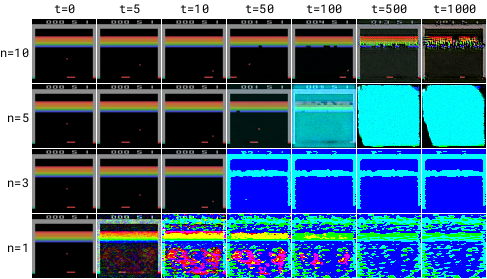
\includegraphics[width=\linewidth]{images/figure__karras_vs_ddpm__ddpm.png}
    \caption{\textsc{ddpm}-based world model trajectories.} \label{fig:denoising_with_ddpm}
  \end{subfigure}%
  \hspace*{\fill}   % maximize separation between the subfigures
  \begin{subfigure}{0.49\textwidth}
    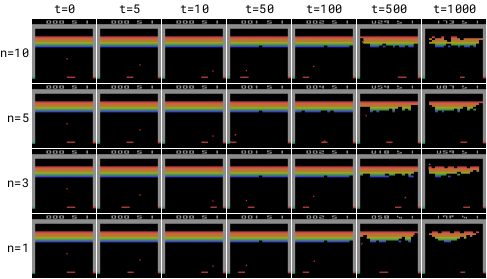
\includegraphics[width=\linewidth]{images/figure__karras_vs_ddpm__karras.png}
    \caption{\textsc{edm}-based world model trajectories.} \label{fig:denoising_with_karras}
  \end{subfigure}%

\caption{Imagined trajectories with diffusion world models based on \textsc{ddpm} (left) and \textsc{edm} (right). The initial observation at $t=0$ is common, and each row corresponds to a decreasing number of denoising steps $n$. We observe that \textsc{ddpm}-based generation suffers from compounding error, and that the smaller the number of denoising steps, the faster the error accumulates. In contrast, our \textsc{edm}-based world model appears much more stable, even for $n=1$.\vspace{-5mm}}
\label{fig:denoising_trajectories} 
\end{figure}
% %%%%%%%%%%%%%%%%%%%%%%%

This surprising result is a consequence of the improved training objective described in Equation~\ref{eq:effective_obj}, compared to the simpler noise prediction objective employed by \textsc{ddpm}. While predicting the noise works well for intermediate noise levels, this objective causes the model to learn the identity function when the noise is dominant ($\sigma_{noise}\gg\sigma_{data} \implies \xi_\theta(\x^\tau_{t+1}, y_t^\tau)\to\mathbf{x}^\tau_{t+1}$), where $\xi_\theta$ is the noise prediction network of \textsc{ddpm}. This gives a poor estimate of the score function at the beginning of the sampling procedure, which degrades the generation quality and leads to compounding error.

In contrast, the adaptive mixing of signal and noise employed by \textsc{edm}, described in Section \ref{subsec:practical_dwm}, means that the model is trained to predict the clean image when the noise is dominant ($\sigma_{noise}\gg\sigma_{data} \implies \mathbf{F_\theta}(\mathbf{x}^\tau_{t+1},y_t^\tau)\to\mathbf{x}^0_{t+1}$). This gives a better estimate of the score function in the absence of signal, so the model is able to produce higher quality generations with fewer denoising steps, as illustrated in Figure \ref{fig:denoising_with_karras}.


\subsection{Choice of the number of denoising steps}\label{subsec:denoising_steps}

 While we found that our \textsc{edm}-based world model was very stable with just a single denoising step, as shown for \textit{Breakout} in the last row of Figure \ref{fig:denoising_with_karras}, we discuss here how this choice would limit the visual quality of the model in some cases. We provide more a quantitative analysis in Appendix~\ref{app:denoising_ablation}.

As discussed in Section \ref{subsec:diffusion}, our score model is equivalent to a denoising autoencoder \citep{vincent2008extracting} trained with an $L_2$ reconstruction loss. The optimal single-step prediction is thus the expectation over possible reconstructions for a given noisy input, which can be out of distribution if this posterior distribution is multimodal. While some games like \textit{Breakout} have deterministic transitions that can be accurately modeled with a single denoising step (see Figure \ref{fig:denoising_with_karras}), in some other games partial observability gives rise to multimodal observation distributions. In this case, an iterative solver is necessary to drive the sampling procedure towards a particular mode, as illustrated in the game \textit{Boxing} in Figure \ref{fig:too_optimisitic_4_sure}. As a result, we therefore set $n=3$ in all of our experiments.
\vspace{-2mm}
%%%%%%%%%%%%%%%%%%%%%%%
\begin{figure}[h!]
%\vspace{-6mm}
\begin{center}
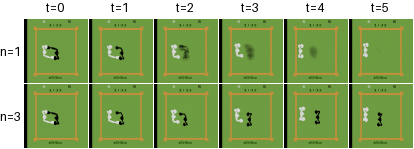
\includegraphics[width=.64\linewidth]{images/figure__blurry_boxing.png}
\caption{Single-step (top row) versus multi-step (bottom row) sampling in \textit{Boxing}. Movements of the black player are unpredictable, so that single-step denoising interpolates between possible outcomes and results in blurry predictions. In contrast, multi-step sampling produces a crisp image by driving the generation towards a particular mode. Interestingly, the policy controls the white player, so his actions are known to the world model. This information removes any ambiguity, and so we observe that both single-step and multi-step sampling correctly predict the white player's position.}
\label{fig:too_optimisitic_4_sure}
\end{center}
\vspace{-4mm}
\end{figure}
%%%%%%%%%%%%%%%%%%%%%%%


\subsection{Qualitative visual comparison with \textsc{iris}}
\label{subsec:comparison_transformers}

We now compare to \textsc{iris} \citep{iris2023}, a well-established world model that uses a discrete autoencoder \citep{vqvae} to convert images to discrete tokens, and composes these tokens over time with an autoregressive transformer \citep{radford2019language}. For fair comparison, we train both world models on the same static datasets of 100k frames collected with expert policies. This comparison is displayed in Figure \ref{fig:iris_vs_diamond} below.

% %%%%%%%%%%%%%%%%%%%%%%%
\begin{figure}[h]
  \begin{subfigure}{0.49\linewidth}
    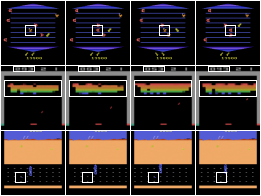
\includegraphics[width=\linewidth]{images/figure__iris_vs_diamond__iris.png}
    \caption{\textsc{iris}} \label{fig:iris_vs_diamond__iris}
  \end{subfigure}%
  \hspace*{\fill}   % maximize separation between the subfigures
  \begin{subfigure}{0.49\textwidth}
    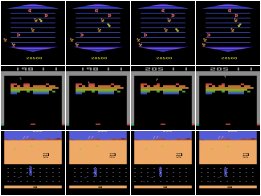
\includegraphics[width=\linewidth]{images/figure__iris_vs_diamond__diamond.png}
    \caption{\textsc{diamond}} \label{fig:iris_vs_diamond__diamond}
  \end{subfigure}%
\caption{Consecutive frames imagined with \textsc{iris} (left) and \textsc{diamond} (right). The white boxes highlight inconsistencies between frames, which we see only arise in trajectories generated with \textsc{iris}. In \textit{Asterix} (top row), an enemy (orange) becomes a reward (red) in the second frame, before reverting to an enemy in the third, and again to a reward in the fourth. In \textit{Breakout} (middle row), the bricks and score are inconsistent between frames. In \textit{Road Runner} (bottom row), the rewards (small blue dots on the road) are inconsistently rendered between frames. None of these inconsistencies occur with \textsc{diamond}. In \textit{Breakout}, the score is even reliably updated by +7 when a red brick is broken\protect\footnotemark.}
\label{fig:iris_vs_diamond}
\end{figure}

\footnotetext{\href{https://en.wikipedia.org/wiki/Breakout_(video_game)\#Gameplay}{\texttt{https://en.wikipedia.org/wiki/Breakout\_(video\_game)\#Gameplay}}}
% %%%%%%%%%%%%%%%%%%%%%%%

We see in Figure \ref{fig:iris_vs_diamond} that the trajectories imagined by \textsc{diamond} are generally of higher visual quality and more faithful to the true environment compared to the trajectories imagined by \textsc{iris}. In particular, the trajectories generated by \textsc{iris} contain visual inconsistencies between frames (highlighted by white boxes), such as enemies being displayed as rewards and vice-versa. These inconsistencies may only represent a few pixels in the generated images, but can have significant consequences for reinforcement learning. For example, since an agent should generally target rewards and avoid enemies, these small visual discrepancies can make it more challenging to learn an optimal policy.

These improvements in the consistency of visual details are generally reflected by greater agent performance on these games, as shown in Table \ref{tab:atari_results_full}. Since the agent component of these methods is similar, this improvement can likely be attributed to the world model. 

Finally, we note that this improvement is not simply the result of increased computation. Both world models are rendering frames at the same resolution ($64\times64$), and \textsc{diamond} requires only 3 NFE per frame compared to 16 NFE per frame for \textsc{iris}. This is further reflected by the fact that \textsc{diamond} has significantly fewer parameters and takes less time to train than \textsc{iris}, as provided in Appendix \ref{app:performance_profile}.
\section{Scaling the diffusion world model to \textit{Counter-Strike: Global Offensive}\protect\footnote{This section was added after NeurIPS acceptance, following community interest in later CS:GO experiments.}}
\label{sec:csgo}

To investigate the ability of \textsc{diamond}'s diffusion world model to learn to model more complex 3D environments, we train the world model in isolation on static data from the popular video game \textit{Counter-Strike: Global Offensive} (CS:GO). We use the \textit{Online} dataset of 5.5M frames (95 hours) of online human gameplay captured at 16Hz from the map \textit{Dust II} by \citet{pearce2022counter}. We randomly hold out 0.5M frames (corresponding to 500 episodes, or 8 hours) for testing, and use the remaining 5M frames (87 hours) for training. There is no reinforcement learning agent or online data collection involved in these experiments.

To reduce the computational cost, we reduce the resolution from $(280\times150)$ to $(56\times30)$ for world modeling. We then introduce a second, smaller diffusion model as an upsampler to improve the generated images at the original resolution \citep{saharia2022image}. We scale the channels of the U-Net to increase the number of parameters from 4M for our Atari models to 381M for our CS:GO model (including 51M for the upsampler). The combined model was trained for 12 days on an RTX 4090. 

Finally, we introduce stochastic sampling and increase the number of denoising steps for the upsampler to 10, which we found to improve the resulting visual quality of the generations, while keeping the dynamics model the same (in particular, still using only 3 denoising steps). This enables a reasonable tradeoff between visual quality and inference cost, with the model running at 10Hz on an RTX 3090. Typical generations of the model are provided in Figure \ref{fig:csgo_grid} below.

%%%%%%%%%%%%%%%%%%%%%%%
\begin{figure}[h]
%\vspace{-6mm}
\begin{center}
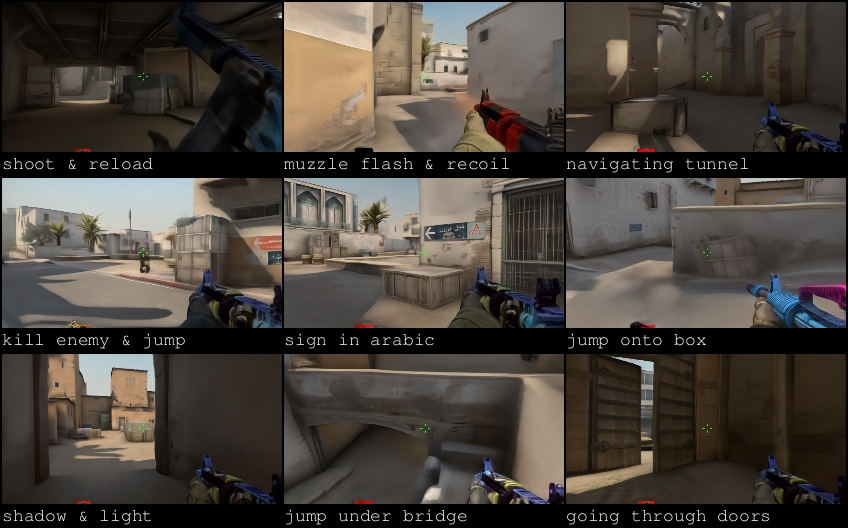
\includegraphics[width=.7\linewidth]{images/csgo_grid.png}
\caption{Images captured from people playing with keyboard and mouse inside \textsc{diamond}'s diffusion world model. This model was trained on $87$ hours of static \textit{Counter-Strike: Global Offensive} (CS:GO) gameplay \citep{pearce2022counter} to produce an interactive neural game engine for the popular in-game map, \textit{Dust II}. Best viewed as videos at \wslink.}
\label{fig:csgo_grid}
\end{center}
\vspace{-4mm}
\end{figure}
%%%%%%%%%%%%%%%%%%%%%%%

We find the model is able to generate stable trajectories over hundreds of timesteps, although is more likely to drift out-of-distribution in less frequently visited areas of the map. Due to the limited memory of the model, approaching walls or losing visibility may cause the model to forget the current state and instead generate a new weapon or area of map. Interestingly, we find the model wrongly enables successive jumps by generalizing the effect of a jump on the geometry of the scene, since multiple jumps do not appear often enough in the training gameplay for the model to learn that mid-air jumps should be ignored. We expect scaling the model and data to address many of these limitations, with the exception of the memory of the model. Quantitative measurements of the capabilities of the CS:GO world model and attempts to address these limitations are left to future work.

% %%%%%%%%%%%%%%%%%%%%%%%
% \begin{wrapfigure}[]{R}{0.55\linewidth}
% \vspace{-5mm}
% \begin{center}
% \centerline{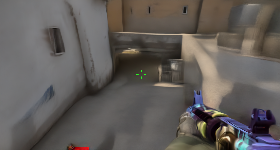
\includegraphics[width=\linewidth]{images/csgo_jump.png}}
% \caption{Looking down at the map after multiple jumps. The model enables multiple jumps by generalizing the effect of a jump on the geometry of the scene, even though only a single jump should be possible. Full video available at \url{https://diamond-wm.github.io}.}
% \label{fig:csgo_jump}
% \end{center}
% \vskip 0in
% \end{wrapfigure}
% %%%%%%%%%%%%%%%%%%%%%%%



% \begin{itemize}
%     \item Motivation: Investigate application of diffusion world model to 3d environment as more complex
%     \item Figure: Example trajectories at different timesteps to show stability (and kb/mouse). Add link to video/website.
%     \item Method: No RL though, things we changed
%     \item Details: In order to reproduce - scaling UNet, discuss actions?, rect not square
%     \item Found stochastic sampling to help
%     \item Results: Playable at 10Hz, long stable trajectories if stay in distribution
%     \item Jump (claim 3d, but be cautious about reasons)
%     \item Limitations + Future work: scaling data/compute, CFG, proper measurements (App J)
% \end{itemize}

% \begin{itemize}
%     \item TODO: Add Generative Game Engine paragraph to related work.
%     \item TODO: update abstract to mention CSGO and website
%     \item TODO: update introduction/conclusion with csgo
%     \item TODO: Update previous CSGO appendix to 'early' experiments
%     \item TODO: Add rebuttal work (training times and DDPM drift) to appendix with mentions from main text
%     \item TODO: Check rebuttal for other promises
% \end{itemize}
\section{Related Work}

\paragraph{Low-precision training}

Techniques introduced to facilitate FP8 training include those covered in \Cref{app:low_precision_and_its_trade_offs} and more \citep{Training_And_Inference_Using_8_Bit,DNNs_With_8_Bit,Mixed_Precision_8_Bit}. These largely concern the quantizing of activations, weights and gradients, though \citep{FP8-LM} also explore FP8 optimizer states and cross-device communication, which we consider interesting avenues of further exploration. Recently, stable training has been demonstrated for the MX family of formats which use a shared block-exponent \citep{MX1,MX2}, and even for the ternary BitNet format \citep{BitNet1,BitNet2,BitNet3}. Again, we consider these formats for follow-up work.
% , though evaluation of these formats and hardware/software support is nascent. Again, we consider examining these formats for \umup\ valuable follow-up work.

\paragraph{Stability features}

Another recent research trend has been the analysis of features that contribute to (or resolve) numerical and algorithmic instability. \citep{Small_Scale_Proxies} show that unstable training dynamics can result from attention logit growth (fixed by QK-norm \citep{Scaling_Vision_Transformers}) and from divergent output logits (fixed by z-loss \citep{Palm}). \citep{Stable_And_Low_Precision_Training} find large feature magnitudes can be avoided by zero-initialization, and loss spikes avoided via a modified AdamW, specifically for low-precision training. \citep{Intriguing_Properties} investigate how pre-training settings affect instabilities revealed during post-training quantization. \citep{Dynamics_Of_Diffusion_Models} apply a similar philosophy to Unit Scaling for the training of diffusion models, to address uncontrolled magnitude changes. Extreme activation values seen in large models \citep{LLM_INT8,SmoothQuant} have been addressed by softmax-clipping \citep{Quantizable_Transformers}, and by the addition of extra terms \citep{Massive_Activations} or tokens \citep{Vision_Transformers_Need_Registers} to bias the attention computation. We do not adopt these features in our experiments to avoid confounding effects, but we expect them to benefit \umup\ and hope to explore their usage.

\paragraph{Learning dynamics}

Several recent efforts have tried to improve \mup\ from different angles.
\citep{Modula} introduces the notion of the \textit{modular norm} over the full weight-space, which like \mup\ aims to ensure stable updates that provide LR transfer, and like \umup\ is implemented via modules designed to ensure stable training.
Challenging the assumptions underpinning \mup, \citep{Scaling_Exponents} explores the notion of \textit{alignment} between parameters and data, demonstrating that other parametrizations with per-layer learning rates can outperform standard \mup. We consider comparing these parametrizations against \umup\ and trying unit-scaled versions valuable future work. Recent applications of \mup\ to the problems of weight sparsity \citep{Sparse_Mup} and structured matrices \citep{Compute_Better_Spent} are also interesting candidates for \umup.

\vspace{-2mm}
\section{Limitations}
\label{sec:limitations}

We identify three main limitations of our work for future research. First, our main evaluation is focused on discrete control environments, and applying \textsc{diamond} to the continuous domain may provide additional insights. Second, the use of frame stacking for conditioning is a minimal mechanism to provide a memory of past observations. Integrating an autoregressive transformer over environment time, using an approach such as \citet{dit2023}, would enable longer-term memory and better scalability. We include an initial investigation into a potential cross-attention architecture in Appendix \ref{app:additonal_experiments}, but found frame-stacking more effective in our early experiments. Third, we leave potential integration of the reward/termination prediction into the diffusion model for future work, since combining these objectives and extracting representations from a diffusion model is not trivial \citep{luo2023dhf, xu2023open} and would make our world model unnecessarily complex.


Copyright traps are unique synthetic sequences injected into original content, enabling its detectability in LLM training. However, traps rely on exact duplication across the content -up to 1,000 times-, making them vulnerable to accidental removal as part of commonly deployed deduplication strategies. We here propose \emph{fuzzy} copyright traps. By replacing a small amount of tokens across duplication, traps become increasingly unlikely to be removed - while we find their detectability to only decrease slightly. In our setup, fuzzy trap sequences with $4$ token replacements in a sequence of $100$ tokens, the mean MIA AUC only drops from $0.90$ to $0.87$ - while now being highly unlikely to be removed by deduplication techniques. 

The fact that fuzzy duplicates are memorized to a similar extent as exact duplicates has implications for LLM memorization and confidentiality. First, we find that in a dataset widely used to train LLMs and study post-hoc memorization, The Pile, many duplicated sequences also have a significant amount of fuzzy duplicates - almost 30\% have at least one, but potentially many more, fuzzy duplicates with as little as 4 mismatched tokens.
We expect this to be a common feature of large text datasets, and to present a major confounding factor in studying memorization using duplicate sequences from such datasets.
Further, our findings highlight additional challenges in training LLMs on private or confidential data. We show that techniques like data deduplication might not be sufficient to eliminate risks of information leakage.

\newpage
 %\section*{Broader Impact}
% This paper considers the training of autonomous agents using a world model. The deployment of autonomous agents in the real world raises safety concerns regarding the potential harm that may be caused by an agent's actions. Training in simulation reduces these risks by reducing the time the agent spends interacting with the environment. However, imperfect world models may lead to unexpected behaviors in the real world. The development of more realistic world models should therefore reduce the risk associated with deploying agents trained in this manner. Additionally, as with all advances in the field of Machine Learning, there are many other potential societal consequences of our work, but none of which we feel must be specifically highlighted here.

\begin{ack}

We would like to thank Andrew Foong, Bálint Máté, Clément Vignac, Maxim Peter, Pedro Sanchez, Rich Turner, Stéphane Nguyen, Tom Lee, Trevor McInroe and Weipu Zhang for insightful discussions and comments.
Adam and Eloi met during an internship at Microsoft Research Cambridge, and would like to thank the Game Intelligence team, including Anssi Kanervisto, Dave Bignell, Gunshi Gupta, Katja Hofmann, Lukas Schäfer, Raluca Georgescu, Sam Devlin, Sergio Valcarcel Macua, Shanzheng Tan, Tabish Rashid, Tarun Gupta, Tim Pearce, and Yuhan Cao, for their support in the early stages of this project, and a great summer.

\end{ack}


\bibliography{main}
\bibliographystyle{apalike}


%%%%%%%%%%%%%%%%%%%%%%%%%%%%%%%%%%%%%%%%%%%%%%%%%%%%%%%%%%%%

\newpage
\appendix
\section{Sampling observations in \textsc{diamond}}
\label{appendix:sampling}

We describe here how we sample an observation $\x_t^0$ from our diffusion world model. We initialize the procedure with a noisy observation $\x_t^\Tau \sim p^{prior}$, and iteratively solve the reverse SDE in Equation \ref{eq:reverse_process} from $\tau = \Tau$ to $\tau = 0$, using the learned score model $\mathbf{S}_\theta(\x_t^\tau, \tau, \x_{<t}^0, a_{<t})$ conditioned on past observations $\x_{<t}^0$ and actions $a_{<t}$. This procedure is illustrated in Figure \ref{fig:architecture}.

In fact, there are many possible sampling methods for a given learned score model $\mathbf{S}_\theta$ \citep{karras2022elucidating}. Notably, \citet{song_sde} introduce a corresponding ``probability flow" ordinary differential equation (ODE), with marginals equivalent to the stochastic process described in Section \ref{subsec:diffusion}. In that case, the solving procedure is deterministic, and the only randomness comes from sampling the initial condition. In practice, this means that for a given score model, we can resort to any ODE or SDE solver, from simple first order methods like Euler (deterministic) and Euler–Maruyama (stochastic) schemes, to higher-order methods like Heun's method \citep{ascher1998computer}. 

Regardless of the choice of solver, each step introduces truncation errors, resulting from the local score approximation and the discretization of the continuous process. Higher order samplers may reduce this truncation error, but come at the cost of additional Number of Function Evaluations (NFE) -- how many forward passes of the network are required to generate a sample. This local error generally scales superlinearly with respect to the step size (for instance Euler's method is $\mathcal{O}(h^2)$ for step size $h$), so increasing the number of denoising steps improves the visual quality of the generated next frame. Therefore, there is a trade-off between visual quality and NFE that directly determines the inference cost of the diffusion world model.


% with t+1 instead of t

% \section{Sampling next observations in \textsc{diamond}}
% \label{appendix:sampling}

% We describe here how we sample a next observation $\x_{t+1}$ from our diffusion world model. We initialize the procedure with a noisy next observation $\x_{t+1}^\Tau \sim p^{prior}$, and iteratively solve the reverse SDE in Equation \ref{eq:reverse_process} from $\tau = \Tau$ to $\tau = 0$, using the learned score model $\mathbf{S}_\theta(\x_{t+1}^\tau, \tau, \x_{\le t}^0, a_{\le t})$ conditioned on past observations $\x_{\le t}^0$ and actions $a_{\le t}$. This procedure is illustrated in Figure \ref{fig:architecture}.

% In fact, there are many possible sampling methods for a given learned score model $S_\theta$ \citep{karras2022elucidating}. Notably, \citet{song_sde} introduce a corresponding ``probability flow" ordinary differential equation (ODE), with equivalent marginals. In that case, the solving procedure is deterministic, and the only randomness comes from sampling the initial condition. In practice, this means that for a given score model, we can resort to any ODE or SDE solver, from simple first order methods like Euler (deterministic) and Euler–Maruyama (stochastic) schemes, to higher-order methods like Heun's method \citep{ascher1998computer}. 

% Regardless of the choice of solver, each step introduces truncation errors, resulting from the local score approximation and the discretization of the continuous process. Higher order samplers may reduce this truncation error, but come at the cost of additional Number of Function Evaluations (NFE) -- how many forward passes of the network are required to generate a sample. This local error generally scales superlinearly with respect to the step size (for instance Euler's method is $\mathcal{O}(h^2)$ for step size $h$), so increasing the number of denoising steps improves the visual quality of the generated next frame. Therefore, there is a trade-off between visual quality and NFE that directly determines the inference cost of the diffusion world model.



\section{Link between DDPM and continuous-time score-based diffusion models}
\label{app:ddpm}

Denoising Diffusion Probabilistic Models (\textsc{ddpm}, \citet{ho2020DDPM}) can be described as a discrete version of the diffusion process introduced in Section \ref{subsec:diffusion}, as described in \citet{song_sde}. The discrete forward process is a Markov chain characterized by a discrete noise schedule $0 < \beta_1, \dots, \beta_i, \dots \beta_N < 1$, and a variance-preserving Gaussian transition kernel,

\begin{equation}
    p(\x^i|\x^{i-1}) = \mathcal{N}(\x^i; \sqrt{1-\beta_i} \x^{i-1}, \beta_i \mathbf{I}).
\end{equation}

In the continuous time limit $N \to \infty$, the Markov chain becomes a diffusion process, and the discrete noise schedule becomes a time-dependent function $\beta(\tau)$. This diffusion process can be described by an SDE with drift coefficient $\mathbf{f}(\x, \tau) = -\frac{1}{2}\beta(\tau)\x$ and diffusion coefficient $g(\tau) = \sqrt{\beta(\tau)}$ \citep{song_sde}. 


\section{\textsc{EDM} network preconditioners and training}
\label{appendix:karras_conditioners}

\citet{karras2022elucidating} use the following preconditioners for normalization and rescaling purposes (as mentioned in Section \ref{subsec:practical_dwm}) to improve network training:

\begin{equation}
    c_{in}^\tau = \frac{1}{\sqrt{\sigma(\tau)^2 + \sigma_{data}^2}}
\end{equation}
\begin{equation}
    c_{out}^\tau = \frac{\sigma(\tau)\sigma_{data}}{\sqrt{\sigma(\tau)^2 + \sigma_{data}^2}}
\end{equation}
\begin{equation}
    c_{noise}^\tau = \frac{1}{4}\log(\sigma(\tau))
\end{equation}
\begin{equation}
    c_{skip}^\tau = \frac{\sigma_{data}^2}{\sigma_{data}^2 + \sigma^2(\tau)},
\end{equation}
where $\sigma_{data}=0.5$.

The noise parameter $\sigma(\tau)$ is sampled to maximize the effectiveness of training as follows:
\begin{equation}
\log(\sigma(\tau))\sim \mathcal{N}(P_{mean}, P_{std}^2),
\end{equation}
where $P_{mean}=-0.4, P_{std}=1.2$. Refer to \citet{karras2022elucidating} for an in-depth analysis.
\newpage
\section{Model architectures}\label{app:architectures}

The diffusion model $\mathbf{D}_\theta$ is a standard U-Net 2D \citep{ronneberger2015unet}, conditioned on the last 4 frames and actions, as well as the diffusion time $\tau$. We use frame stacking for observation conditioning, and adaptive group normalization \citep{adagn} for action and diffusion time conditioning.

The reward/termination model $R_\psi$ layers are shared except for the final prediction heads. The model takes as input a sequence of frames and actions, and forwards it through convolutional residual blocks \citep{He2015} followed by an LSTM cell \citep{a3c,lstm,Gers2000}. Before starting the imagination procedure, we burn-in \citep{r2d2} the conditioning frames and actions to initialize the hidden and cell states of the LSTM. 

The weights of the policy $\pi_\phi$ and value network $V_\phi$ are shared except for the last layer. In the following, we refer to $(\pi,V)_\phi$ as the "actor-critic" network, even though $V$ is technically a state-value network, not a critic. This network takes as input a frame, and forwards it through convolutional trunk followed by an LSTM cell. The convolutional trunk consists of four residual blocks and 2x2 max-pooling with stride 2. The main path of the residual blocks consists of a group normalization \citep{groupnorm} layer, a SiLU activation \citep{elfwing2018sigmoid}, and a 3x3 convolution with stride 1 and padding 1. Before starting the imagination procedure, we burn-in the conditioning frames to initialize the hidden and cell states of the LSTM. 


Please refer to Table \ref{tbl_architecture} below for hyperparameter values, and to Algorithm \ref{alg:diamond} for a detailed summary of the training procedure. 

\vspace{1cm}

\begin{table}[h!]
\caption{Architecture details for \textsc{diamond}.}
\label{tbl_architecture}
\begin{center}
% \resizebox{0.4 \columnwidth}{!}{
\begin{tabular}{ l c }
\multicolumn{1}{c}{\textbf{Hyperparameter}}  & \multicolumn{1}{c}{\textbf{Value}} \\ 

\hline \\

% \hline \\
\\
\multicolumn{2}{l}{\textbf{Diffusion Model ($\mathbf{D}_\theta$)}} \\
% Number of conditioning observations/actions ($L$) & 4 \\
Observation conditioning mechanism & Frame stacking \\
Action conditioning mechanism & Adaptive Group Normalization \\
Diffusion time conditioning mechanism & Adaptive Group Normalization \\
Residual blocks layers & [2, 2, 2, 2] \\
Residual blocks channels & [64, 64, 64, 64] \\
Residual blocks conditioning dimension & 256 \\

% \hline \\
\\
\multicolumn{2}{l}{\textbf{Reward/Termination Model ($R_\psi$)}} \\
Action conditioning mechanisms & Adaptive Group Normalization \\
Residual blocks layers & [2, 2, 2, 2] \\
Residual blocks channels & [32, 32, 32, 32] \\
Residual blocks conditioning dimension & 128 \\
LSTM dimension & 512 \\ 
% Burn-in length ($B_{rt}$), set as $B_{rt} = L$ in practice & 4 \\ 
% Training sequence length ($B_{rt} + H$) & 19 \\

% \hline \\
\\
\multicolumn{2}{l}{\textbf{Actor-Critic Model ($\pi_\phi$ and $V_\phi$)}} \\
Residual blocks layers & [1, 1, 1, 1] \\
Residual blocks channels & [32, 32, 64, 64] \\
LSTM dimension & 512 \\ 
% Burn-in length ($B_{ac}$), set as $B_{ac} = L$ in practice & 4 \\


\end{tabular}
% }
\end{center}
\end{table}

\newpage
\section{Training hyperparameters}
\label{app:hyperparams}

\vspace{1cm}

\begin{table}[h!]
\caption{Hyperparameters for \textsc{diamond}.}
\label{tbl_atari_hypers}
\begin{center}
% \resizebox{0.4 \columnwidth}{!}{
\begin{tabular}{ l c }
\multicolumn{1}{c}{\textbf{Hyperparameter}}  & \multicolumn{1}{c}{\textbf{Value}} \\ 

\hline \\

\multicolumn{2}{l}{\textbf{Training loop}} \\
Number of epochs & 1000 \\
Training steps per epoch & 400 \\
Batch size & 32 \\
Environment steps per epoch & 100 \\
Epsilon (greedy) for collection & 0.01 \\

\\

\multicolumn{2}{l}{\textbf{RL hyperparameters}} \\
Imagination horizon ($H$) & 15 \\
Discount factor ($\gamma$) &  0.985 \\ 
Entropy weight ($\eta$) & 0.001 \\ 
$\lambda$-returns coefficient ($\lambda$) & 0.95 \\

\\

\multicolumn{2}{l}{\textbf{Sequence construction during training}} \\
For $\mathbf{D}_\theta$, number of conditioning observations and actions ($L$) & 4 \\
For $R_\psi$, burn-in length ($B_{R}$), set to $L$ in practice & 4 \\ 
For $R_\psi$, training sequence length ($B_{R} + H$) & 19 \\
For $\pi_\phi$ and $V_\phi$, burn-in length ($B_{\pi,V}$), set to $L$ in practice & 4 \\

\\
\multicolumn{2}{l}{\textbf{Optimization}} \\
Optimizer & AdamW \\
Learning rate & 1e-4 \\
Epsilon & 1e-8 \\
Weight decay ($\mathbf{D}_\theta$) & 1e-2 \\
Weight decay ($R_\psi$) & 1e-2 \\
Weight decay ($\pi_\phi$ and $V_\phi$)  & 0 \\

% \hline \\
\\
\multicolumn{2}{l}{\textbf{Diffusion Sampling}} \\
Method &  Euler \\
Number of steps & 3 \\

\\
\multicolumn{2}{l}{\textbf{Environment}} \\
Image observation dimensions & 64$\times$64$\times$3 \\
Action space & Discrete (up to 18 actions) \\
Frameskip & 4 \\
Max noop & 30 \\
Termination on life loss & True \\
Reward clipping & $\{-1, 0, 1\}$ \\

\end{tabular}
% }
\end{center}
\end{table}

\newpage
\section{Reinforcement learning objectives}
\label{appendix:rl_actor_critic}

In what follows, we note $\x_t$, $r_t$ and $d_t$ the observations, rewards, and boolean episode terminations predicted by our world model. We note $H$ the imagination horizon, $V_\phi$ the value network, $\pi_\phi$ the policy network, and $a_t$ the actions taken by the policy within the world model. 

We use $\lambda$-returns to balance bias and variance as the regression target for the value network. Given an imagined trajectory of length $H$, we can define the $\lambda$-return recursively as follows,

\begin{equation}
\Lambda_t = 
\begin{cases}
    r_t + \gamma (1 - d_t) \Big[ (1 - \lambda) V_\phi(\x_{t+1}) + \lambda \Lambda_{t+1} \Big]   & \text{if}\quad t < H \\
    V_\phi(\x_H)                                                                                            & \text{if}\quad t = H. \\
\end{cases}
\end{equation}

The value network $V_\phi$ is trained to minimize $\mathcal{L}_V(\phi)$, the expected squared difference with $\lambda$-returns over imagined trajectories,

\begin{equation}
\mathcal{L}_V(\phi) = \mathbb{E}_{\pi_\phi} \left[ \sum_{t=0}^{H-1} \big( V_\phi(\x_t) - \mathrm{sg} ( \Lambda_t ) \big)^2 \right],
\end{equation}

where $\operatorname{sg}(\cdot)$ denotes the gradient stopping operation, meaning that the target is a constant in the gradient-based optimization, as classically established in the literature \citep{mnih2015dqn,hafner2021mastering,iris2023}.

As we can generate large amounts of on-policy trajectories in imagination, we use a simple \textsc{reinforce} objective to train the policy, with the value $V_\phi(\x_t)$ as a baseline to reduce the variance of the gradients \citep{sutton2018reinforcement}. The policy is trained to minimize the following objective, combining \textsc{reinforce} and a weighted entropy maximization objective to maintain sufficient exploration,

\begin{equation}
\mathcal{L}_\pi(\phi) = - \mathbb{E}_{\pi_\phi} \left[ \sum_{t=0}^{H-1} \log\left(\pi_\phi\left(a_t \mid \x_{\le t}\right)\right) \operatorname{sg}\left(\Lambda_t - V_\phi\left(\x_t\right)\right) + \eta \operatorname{\mathcal{H}}\left(\pi_\phi \left(a_t \mid \x_{\le t} \right) \right)\right].
\end{equation}

\vspace{1cm}


\newpage
% ALGORITHM STYLE -- Released 8 April 1996
%    for LaTeX-2e
% Copyright -- 1994 Peter Williams
% E-mail Peter.Williams@dsto.defence.gov.au
\NeedsTeXFormat{LaTeX2e}
\ProvidesPackage{algorithm}
\typeout{Document Style `algorithm' - floating environment}

\RequirePackage{float}
\RequirePackage{ifthen}
\newcommand{\ALG@within}{nothing}
\newboolean{ALG@within}
\setboolean{ALG@within}{false}
\newcommand{\ALG@floatstyle}{ruled}
\newcommand{\ALG@name}{Algorithm}
\newcommand{\listalgorithmname}{List of \ALG@name s}

% Declare Options
% first appearance
\DeclareOption{plain}{
  \renewcommand{\ALG@floatstyle}{plain}
}
\DeclareOption{ruled}{
  \renewcommand{\ALG@floatstyle}{ruled}
}
\DeclareOption{boxed}{
  \renewcommand{\ALG@floatstyle}{boxed}
}
% then numbering convention
\DeclareOption{part}{
  \renewcommand{\ALG@within}{part}
  \setboolean{ALG@within}{true}
}
\DeclareOption{chapter}{
  \renewcommand{\ALG@within}{chapter}
  \setboolean{ALG@within}{true}
}
\DeclareOption{section}{
  \renewcommand{\ALG@within}{section}
  \setboolean{ALG@within}{true}
}
\DeclareOption{subsection}{
  \renewcommand{\ALG@within}{subsection}
  \setboolean{ALG@within}{true}
}
\DeclareOption{subsubsection}{
  \renewcommand{\ALG@within}{subsubsection}
  \setboolean{ALG@within}{true}
}
\DeclareOption{nothing}{
  \renewcommand{\ALG@within}{nothing}
  \setboolean{ALG@within}{true}
}
\DeclareOption*{\edef\ALG@name{\CurrentOption}}

% ALGORITHM
%
\ProcessOptions
\floatstyle{\ALG@floatstyle}
\ifthenelse{\boolean{ALG@within}}{
  \ifthenelse{\equal{\ALG@within}{part}}
     {\newfloat{algorithm}{htbp}{loa}[part]}{}
  \ifthenelse{\equal{\ALG@within}{chapter}}
     {\newfloat{algorithm}{htbp}{loa}[chapter]}{}
  \ifthenelse{\equal{\ALG@within}{section}}
     {\newfloat{algorithm}{htbp}{loa}[section]}{}
  \ifthenelse{\equal{\ALG@within}{subsection}}
     {\newfloat{algorithm}{htbp}{loa}[subsection]}{}
  \ifthenelse{\equal{\ALG@within}{subsubsection}}
     {\newfloat{algorithm}{htbp}{loa}[subsubsection]}{}
  \ifthenelse{\equal{\ALG@within}{nothing}}
     {\newfloat{algorithm}{htbp}{loa}}{}
}{
  \newfloat{algorithm}{htbp}{loa}
}
\floatname{algorithm}{\ALG@name}

\newcommand{\listofalgorithms}{\listof{algorithm}{\listalgorithmname}}


\newpage
\section{Additional performance comparisons}
\label{app:performance_profile}

We provide performance profiles \citep{agarwal2021deep} for \textsc{diamond} and baselines below. % We see that \textsc{diamond} outperforms the baselines in terms of the fraction of runs above a given human normalized score for a range of scores.

%%%%%%%%%%%%%%%%%%%%%%%
\begin{figure}[h!]
\vskip 0.2in
\begin{center}
\centerline{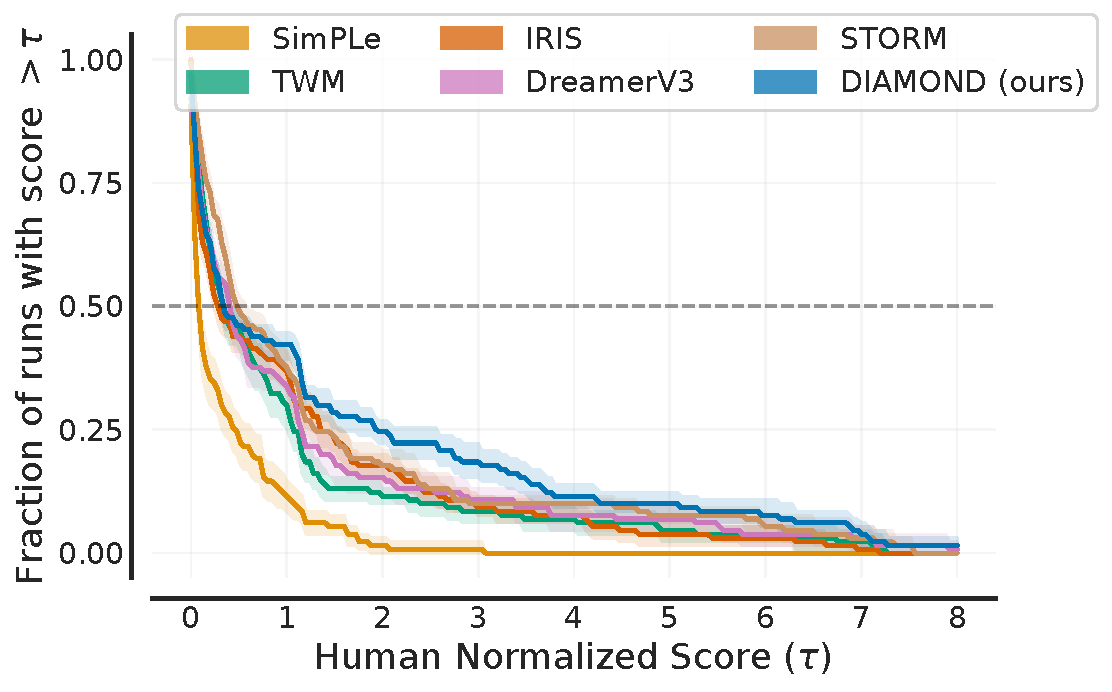
\includegraphics[width=.7\columnwidth]{images/performance_profile.pdf}}
\caption{Performance profiles, i.e. fraction of runs above a given human normalized score.}
\label{fig:results_performance_profile}
\end{center}
\vskip 0.2in
\end{figure}
%%%%%%%%%%%%%%%%%%%%%%%

As additional angles of comparison, we also provide parameter counts and approximate training times for \textsc{iris}, DreamerV3 and \textsc{diamond} in Table \ref{tab:training_time} below. We see that \textsc{diamond} has the highest mean HNS, with fewer parameters than both \textsc{iris} and DreamerV3. \textsc{diamond} also trains faster than \textsc{iris}, although is slower than DreamerV3. 

\begin{table}[h]
\caption{Number of parameters, training time, and mean human-normalized score (HNS).}
\label{tab:training_time}
\begin{center}
\begin{tabular}{lcccc}
\hline
    & \textsc{iris} & DreamerV3 & \textsc{diamond} (ours) & \\ \hline
\#parameters (↓)        & 30M       & 18M            & \textbf{13M}   &  \\
Training days (↓) & 4.1       & \textbf{\textless 1}   & 2.9   &  \\
Mean HNS (↑)            & 1.046     & 1.097          & \textbf{1.459} &  \\ \hline
\end{tabular}
\end{center}
\end{table}



A full training time profile for \textsc{diamond} is provided in Appendix~\ref{app:profiling}.
\newpage
\section{Training time profile}\label{app:profiling}

Table~\ref{tab:profiling} provides a full training time profile for \textsc{diamond}.

\begin{table}[h!]
\caption{Detailed breakdown of training time. Profiling performed using a Nvidia RTX 4090 with the default hyperparameters specified in Appendices \ref{app:architectures} and \ref{app:hyperparams} These profiling measures are representative, since exact durations will depend on the machine, the environment, and the training stage.}
\label{tab:profiling}
\begin{center}

\scalebox{1.0}{

\begin{tabular}{|>{\raggedright\arraybackslash}p{7cm}|>{\raggedleft\arraybackslash}p{2cm}|>{\raggedleft\arraybackslash}p{3.5cm}|}
    \hline
    \textbf{Single update} & \textbf{Time (ms)} & \textbf{Detail (ms)} \\
    \hline
    Total & $543$ & $88 + 115 + 340$\\
    \hspace{0.5cm} Diffusion model update & $88$ & - \\
    \hspace{0.5cm} Reward/Termination model update & $115$ & - \\
    \hspace{0.5cm} Actor-Critic model update & $340$ & $15 \times 20.4 + 34$\\
    \hspace{1cm} Imagination step (x 15) & $20.4$ & $12.7 + 7.0 + 0.7$ \\
    \hspace{1.5cm} Next observation prediction & $12.7$ & $3 \times 4.2$ \\
    \hspace{2cm} Denoising step (x 3) & $4.2$ & - \\
    \hspace{1.5cm} Reward/Termination prediction & $7.0$ & - \\
    \hspace{1.5cm} Action prediction & $0.7$ & - \\
    \hspace{1cm} Loss computation and backward & $34$ & - \\
    \hline
    \textbf{Epoch} & \textbf{Time (s)} & \textbf{Detail (s)} \\
    \hline
    Total & $217$ & $35 + 46 + 136$ \\
    \hspace{0.5cm} Diffusion model & $35$ & $400 \times 88 \times  10^{-3}$ \\
    \hspace{0.5cm} Reward/Termination model & $46$ & $400 \times 115 \times  10^{-3}$ \\
    \hspace{0.5cm} Actor-Critic model & $136$ & $400 \times 340 \times  10^{-3}$ \\
    \hline
    \textbf{Run} & \textbf{Time (days)} & \textbf{Detail (days)} \\
    \hline
    Total & $2.9$ & $2.5 + 0.4$ \\
    \hspace{0.5cm} Training time & $2.5$ & $1000 \times 217 / (24 \times 3600)$ \\
    \hspace{0.5cm} Other (collection, evaluation, checkpointing) & $0.4$ & - \\
    \hline
\end{tabular}

}

\end{center}
\end{table}
\label{tab:r}
%% \section{Scope and limitations}
% We frame many existing algorithms for composing models in terms of probabilistic programming. While this suggests the possibility of applying a variety of existing inference and train-time techniques to the resulting models, the present work does not evaluate methods beyond rejection sampling.
% 
% A challenge applying cascades in practice is the difficulty of probabilistic inference in models with string-valued variables. Previous work in particle based inference for probabilistic programs provides some hope in this direction \citep{anglican}.

% This perspective opens up exciting new directions in applications of language models, and in foundation models more generally.
% Existing fine-tuning methods can be described with a principled probabilistic programming language formalism representing structured distributions known as LM Cascades. This defines the distribution on the string-valued output of a large language model, the compositions of which may be adapted as specific inference algorithms underpinning various applications. 


% efficiency / expense
% We don't actually explore specific inference methods
% Hint of 
% hints @ lots of possibilities, explores very few of them
% - multimodality
% - train/test time inference beyond rejection sampling
% - tool use
\newpage
\section{Broader comparison to model-free and search-based methods}
\label{app:additonal_baselines}

Table \ref{tab:atari_results_other_baselines} provides scores for model-free and search-based methods, including the current best performing methods on the Atari 100k benchmark, EfficientZero \citep{ye2021efficientzero} and \textsc{bbf} \citep{schwarzer2023bigger}. Both of these methods use approaches that are out of scope of our approach, such as computationally expensive lookahead Monte-Carlo tree search for EfficientZero, and using periodic network resets in combination with hyperparameter scheduling for \textsc{bbf}. We see that while the use of lookahead search and more advanced reinforcement learning techniques (for EfficientZero \citep{ye2021efficientzero} and \textsc{bbf} \citep{schwarzer2023bigger} respectively) can still provide greater performance overall, \textsc{diamond} promisingly still outperforms these methods on some games.

\begin{table*}[h]
    \caption{Raw scores and human-normalized metrics for search-based and model-free methods.}
    \label{tab:atari_results_other_baselines}
\begin{center}
\begin{small}
\centering
\scalebox{0.86}{
\centering

\begin{tabular}{lrr rrrrrr}
\toprule
\multicolumn{2}{c}{} & \multicolumn{2}{c}{Search-based} & \multicolumn{4}{c}{Model-free} \\
\cmidrule(lr){3-4} \cmidrule(lr){5-8}
%%%%%%%%%%%%%%%%%%%%%%%%%%%%%%%%%%%%%%%%%%%%%%%%%%%%%%%%%%%%%%%%%%%%
Game                 &  Human     &  MuZero    &  EfficientZero      &  CURL     &  SPR       &  SR-SPR              &  BBF                &  \textsc{diamond} (ours)  \\
\midrule
Alien                &  7127.7    &  530.0     &  808.5              &  711.0    &  841.9     &  1107.8              &  \textbf{1173.2}    &  744.1                    \\
Amidar               &  1719.5    &  38.8      &  148.6              &  113.7    &  179.7     &  203.4               &  \textbf{244.6}     &  225.8                    \\
Assault              &  742.0     &  500.1     &  1263.1             &  500.9    &  565.6     &  1088.9              &  \textbf{2098.5}    &  1526.4                   \\
Asterix              &  8503.3    &  1734.0    &  \textbf{25557.8}   &  567.2    &  962.5     &  903.1               &  3946.1             &  3698.5                   \\
BankHeist            &  753.1     &  192.5     &  351.0              &  65.3     &  345.4     &  531.7               &  \textbf{732.9}     &  19.7                     \\
BattleZone           &  37187.5   &  7687.5    &  13871.2            &  8997.8   &  14834.1   &  17671.0             &  \textbf{24459.8}   &  4702.0                   \\
Boxing               &  12.1      &  15.1      &  52.7               &  0.9      &  35.7      &  45.8                &  85.8               &  \textbf{86.9}            \\
Breakout             &  30.5      &  48.0      &  \textbf{414.1}     &  2.6      &  19.6      &  25.5                &  370.6              &  132.5                    \\
ChopperCommand       &  7387.8    &  1350.0    &  1117.3             &  783.5    &  946.3     &  2362.1              &  \textbf{7549.3}    &  1369.8                   \\
CrazyClimber         &  35829.4   &  56937.0   &  83940.2            &  9154.4   &  36700.5   &  45544.1             &  58431.8            &  \textbf{99167.8}         \\
DemonAttack          &  1971.0    &  3527.0    &  13003.9            &  646.5    &  517.6     &  2814.4              &  \textbf{13341.4}   &  288.1                    \\
Freeway              &  29.6      &  21.8      &  21.8               &  28.3     &  19.3      &  25.4                &  25.5               &  \textbf{33.3}            \\
Frostbite            &  4334.7    &  255.0     &  296.3              &  1226.5   &  1170.7    &  \textbf{2584.8}     &  2384.8             &  274.1                    \\
Gopher               &  2412.5    &  1256.0    &  3260.3             &  400.9    &  660.6     &  712.4               &  1331.2             &  \textbf{5897.9}          \\
Hero                 &  30826.4   &  3095.0    &  \textbf{9315.9}    &  4987.7   &  5858.6    &  8524.0              &  7818.6             &  5621.8                   \\
Jamesbond            &  302.8     &  87.5      &  517.0              &  331.0    &  366.5     &  389.1               &  \textbf{1129.6}    &  427.4                    \\
Kangaroo             &  3035.0    &  62.5      &  724.1              &  740.2    &  3617.4    &  3631.7              &  \textbf{6614.7}    &  5382.2                   \\
Krull                &  2665.5    &  4890.8    &  5663.3             &  3049.2   &  3681.6    &  5911.8              &  8223.4             &  \textbf{8610.1}          \\
KungFuMaster         &  22736.3   &  18813.0   &  \textbf{30944.8}   &  8155.6   &  14783.2   &  18649.4             &  18991.7            &  18713.6                  \\
MsPacman             &  6951.6    &  1265.6    &  1281.2             &  1064.0   &  1318.4    &  1574.1              &  \textbf{2008.3}    &  1958.2                   \\
Pong                 &  14.6      &  -6.7      &  20.1               &  -18.5    &  -5.4      &  2.9                 &  16.7               &  \textbf{20.4}            \\
PrivateEye           &  69571.3   &  56.3      &  96.7               &  81.9     &  86.0      &  97.9                &  40.5               &  \textbf{114.3}           \\
Qbert                &  13455.0   &  3952.0    &  \textbf{13781.9}   &  727.0    &  866.3     &  4044.1              &  4447.1             &  4499.3                   \\
RoadRunner           &  7845.0    &  2500.0    &  17751.3            &  5006.1   &  12213.1   &  13463.4             &  \textbf{33426.8}   &  20673.2                  \\
Seaquest             &  42054.7   &  208.0     &  1100.2             &  315.2    &  558.1     &  819.0               &  \textbf{1232.5}    &  551.2                    \\
UpNDown              &  11693.2   &  2896.9    &  17264.2            &  2646.4   &  10859.2   &  \textbf{112450.3}   &  12101.7            &  3856.3                   \\
\midrule
\#Superhuman (↑)     &  N/A       &  5         &  \textbf{14}        &  2        &  6         &  9                   &  12                 &  11                       \\
Mean (↑)             &  1.000     &  0.562     &  1.943              &  0.261    &  0.616     &  1.271               &  \textbf{2.247}     &  1.459                    \\
IQM (↑)              &  1.000     &  0.288     &  1.047              &  0.113    &  0.337     &  0.700               &  \textbf{1.139}     &  0.641                    \\
%%%%%%%%%%%%%%%%%%%%%%%%%%%%%%%%%%%%%%%%%%%%%%%%%%%%%%%%%%%%%%%%%%

\bottomrule
\end{tabular}
 }
\end{small}
\end{center}
%\vspace{-0.02\linewidth}
\end{table*}

\newpage
\section{Quantitative analysis of autoregressive model drift}\label{app:ddpm_drift}

Figure~\ref{fig:ddpm_drift} provides a quantitative measure of the compounding error demonstrated qualitatively in Figure~\ref{fig:denoising_trajectories} for DDPM and EDM based world models.

\begin{figure}[h!]
\begin{center}
\centerline{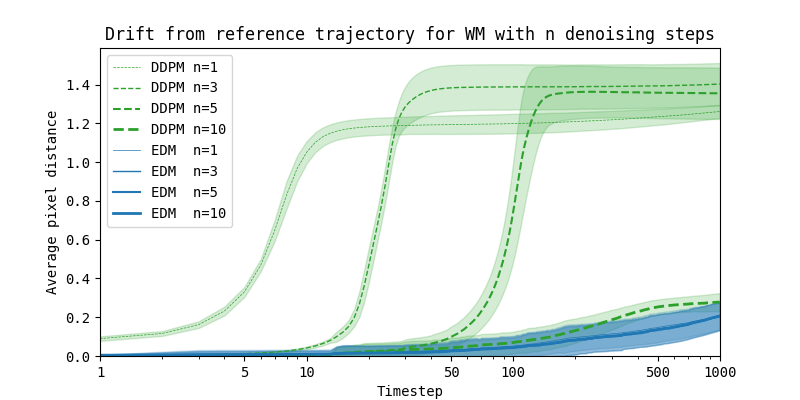
\includegraphics[width=\columnwidth]{images/drift.png}}
\caption{Average pixel drift between an imagined trajectory and the corresponding reference trajectory collected with an expert in \textit{Breakout}. The trajectories are each 1000 timesteps, starting from the same frame and following the same sequence of actions. Each line displays the average and shaded standard deviation of 400 reference trajectories held out from training data. DDPM becomes more stable with increasing number of denoising steps, but is less stable than 1-step EDM, even with 10 denoising steps. The drift we observe for EDM corresponds to differences in the imagined trajectory rather than a pathological color shift as we see in Figure 3a.}
\label{fig:ddpm_drift}
\end{center}
\end{figure}
\section{Quantitative ablation on reducing the number of denoising steps}\label{app:denoising_ablation}

Table~\ref{tab:ablation_rl_1_step} provides a quantitative ablation of the effect of reducing the number of denoising steps used for our EDM diffusion world model from 3 (used for Table~\ref{tab:atari_results_full}) to 1, for \textsc{diamond}'s 10 highest performing games. Note that the 1-step results correspond to a single seed only so will have higher variance. Nonetheless, these results provide some signal that agents trained with 1 denoising step perform worse than our default choice of 3, particularly for the game \textit{Boxing}, despite the apparent similarity in Figure~\ref{fig:ddpm_drift}. This additional evidence supports our qualitative analysis in Section \ref{subsec:denoising_steps}.

\begin{table*}[h]
\caption{Quantitative ablation on reducing the number of denoising steps from 3 (default) to 1.}
\label{tab:ablation_rl_1_step}
\begin{center}
\begin{small}
\centering
\scalebox{1.0}{
\centering
\begin{tabular}{lrr rr}
\toprule
%\multicolumn{3}{c}{} & \multicolumn{2}{c}{Model-free} & \multicolumn{5}{c}{Imagination-based} \\
%\cmidrule(lr){4-5} \cmidrule(lr){6-11}

%%%%%%%%%%%%%%%%%%%%%%%%%%%%%%%%%%%%%%%%%%%%%%%%%%%%%%%%%%%%%%%%%%%%
Game                 &  Random    &  Human     &  \textsc{diamond} ($n=3$)  & \textsc{diamond} ($n=1$)  \\
\midrule
Amidar               &  5.8       &  1719.5    &  \textbf{225.8}           & 191.8 \\
Assault              &  222.4     &  742.0     &  \textbf{1526.4}          & 782.5 \\
Asterix              &  210.0     &  8503.3    &          3698.5           & \textbf{6687.0} \\
Boxing               &  0.1       &  12.1      &  \textbf{86.9}            & 41.9            \\
Breakout             &  1.7       &  30.5      &  \textbf{132.5}           & 50.8            \\
CrazyClimber         &  10780.5   &  35829.4   &  \textbf{99167.8}         & 87233.0         \\
Kangaroo             &  52.0      &  3035.0    &  \textbf{5382.2}          & 1710.0          \\
Krull                &  1598.0    &  2665.5    &          8610.1           & \textbf{9105.1} \\
Pong                 &  -20.7     &  14.6      &          20.4             & \textbf{20.9}   \\
RoadRunner           &  11.5      &  7845.0    &  \textbf{20673.2}         & 5084.0          \\
\midrule
Mean HNS (↑)         &  0.000     &  1.000     &  \textbf{3.052}           & 1.962           \\
%%%%%%%%%%%%%%%%%%%%%%%%%%%%%%%%%%%%%%%%%%%%%%%%%%%%%%%%%%%%%%%%%%

\bottomrule
\end{tabular}
 }
\end{small}
\end{center}
%\vspace{-1cm}
\end{table*}
\newpage
% \section{Data Diversity Leads to Generalization}
\label{sec:data_diversity}
Our experiments thus far have linked training stability to rule commitment. In this section, we will show that models can, in fact, stabilize without a systematic rule---if they memorize their training instead. Less diverse training data produces models that stabilize through memorization, whereas more diverse training data produces models that commit to systematic rules. Furthermore, mirroring our previous findings in data complexity, intermediate levels of data diversity lead to highly unstable runs even when all examples induce the same rule. 
\subsection{Measuring Data Diversity}
\label{sec:data_diveristy}

We define the diversity of a dataset according to the syntactic similarity between different examples. 
We measure a sentence pair's similarity by the tree-edit distance (TED) of their latent tree representations \citep{Chomsky2015-bg}. When two sentences share the same syntax tree, transforming one into the other requires only leaf-node (i.e., vocabulary) changes. For example, \textit{My unicorn entertains her tyrannosaurus}, and, \textit{Your zebra eats some apples}, have different vocabulary but identical syntax trees. We define a dataset's diversity as the number of unique syntactic trees it contains. Similar methods are used to measure diversity in both natural language \citep{Huang2023-ab, Gao2024-fi, Ramirez2022-mx} and code \citep{Song2024-cg}. 

\subsection{Diversity and stability}
\label{sec:inverse}

We will next show that when the model is exposed to fewer unique syntax trees during training, it memorizes their patterns without reliably applying rules to unseen structures. We demonstrate the effect by designing datasets to induce either hierarchical or linear generalization and then adjusting adjusting the syntactic diversity of representative examples. Whichever rule is induced, diversity imposes three distinct regimes: stable memorization behavior at low diversity, stable generalization behavior at high diversity, and unstable behavior at intermediate levels. This transition, from stable to unstable to back to stable, forms a U-shaped curve of stability with respect to dataset diversity.

\paragraph{Hierarchy-inducing data}  
We first control data diversity on datasets that induce hierarchical generalization in QF. We construct variations of the QF training data with different levels of syntactic diversity. Each constructed training set includes 50K question samples and 50K center embedding declarations, while varying the syntactic diversity of the declaration examples. We train 50 random seeds for each modified training set and measure intra-run instability with total variation (see \ref{sec:tv_def}). To assess rule commitment, we report the proportion of runs achieving generalization accuracy either >95\% or < 5\%, indicating a commitment to either rule (here, hierarchical rule is preferred).


Figure \ref{fig:data_diversity_uscale} (\textit{left}) shows an inverse U-shaped relationship between data diversity and training instability, revealing three distinct regimes. Low-diversity data leads to the \textbf{memorization regime}, where training is stable but the model fails to commit to a rule. In Appendix \ref{appdx:memorizaition}, we confirm that models in this low-diversity regime apply the hierarchical rule to syntax structures memorized during training, but cannot extrapolate the rule to unseen  structures. High-diversity data leads to the \textbf{hierarchical generalization regime}, where training stabilizes because models commit to the hierarchical rule. In the mid-diversity \textbf{unstable regime}, the lack of data diversity hinders the likelihood of fully commiting to a rule but the data is too diverse to memorize easily. Overall, with insufficient diversity, relatively few runs learn to apply the hierarchical rule across all examples.

\paragraph{Linearity-inducing data} 
In Figure \ref{fig:intra_inter_variance} (\textit{right}), the model has a strong preference to apply the linear rule OOD when the training data contains 99\% linearity-inducing data (i.e., right branching sentences). However, Figure \ref{fig:grokking_selection} shows that when the training data contains \textit{exclusively} right-branching sentences, models do not consistently follow any systematic rule (further details in  Appendix \ref{sec:simple_mixin}). We can use data diversity to explain the failure to commit to a rule from exclusively right-branching examples: right-branching sentences lack syntactic variation, as the main auxiliary always follows the subject noun. This lack of syntax diversity prevents rule extrapolation. By introducing center embeddings in just 1\% of sentences, we introduce the diversity necessary to learn a systematic generalization rule. 

To confirm that data diversity is also key to rule commitment for when data is mostly linearity-inducing, we create variations of QF training data with 50K questions and 50K declarations, including 99\% right-branching and 1\% center-embedded sentences. We control the diversity of \textit{center-embedded} sentences as before and use the proportion of runs achieving generalization accuracy either above 95\% or below 5\% to quantify the likelihood of committing to any rule (in this data setting, linear rule is preferred). Figure \ref{fig:data_diversity_uscale} (\textit{right}) shows that training is least stable at intermediate levels of diversity, again providing three regimes: the memorization, unstable, and \textbf{linear generalization regime}.


\begin{figure}[t]
    \centering
    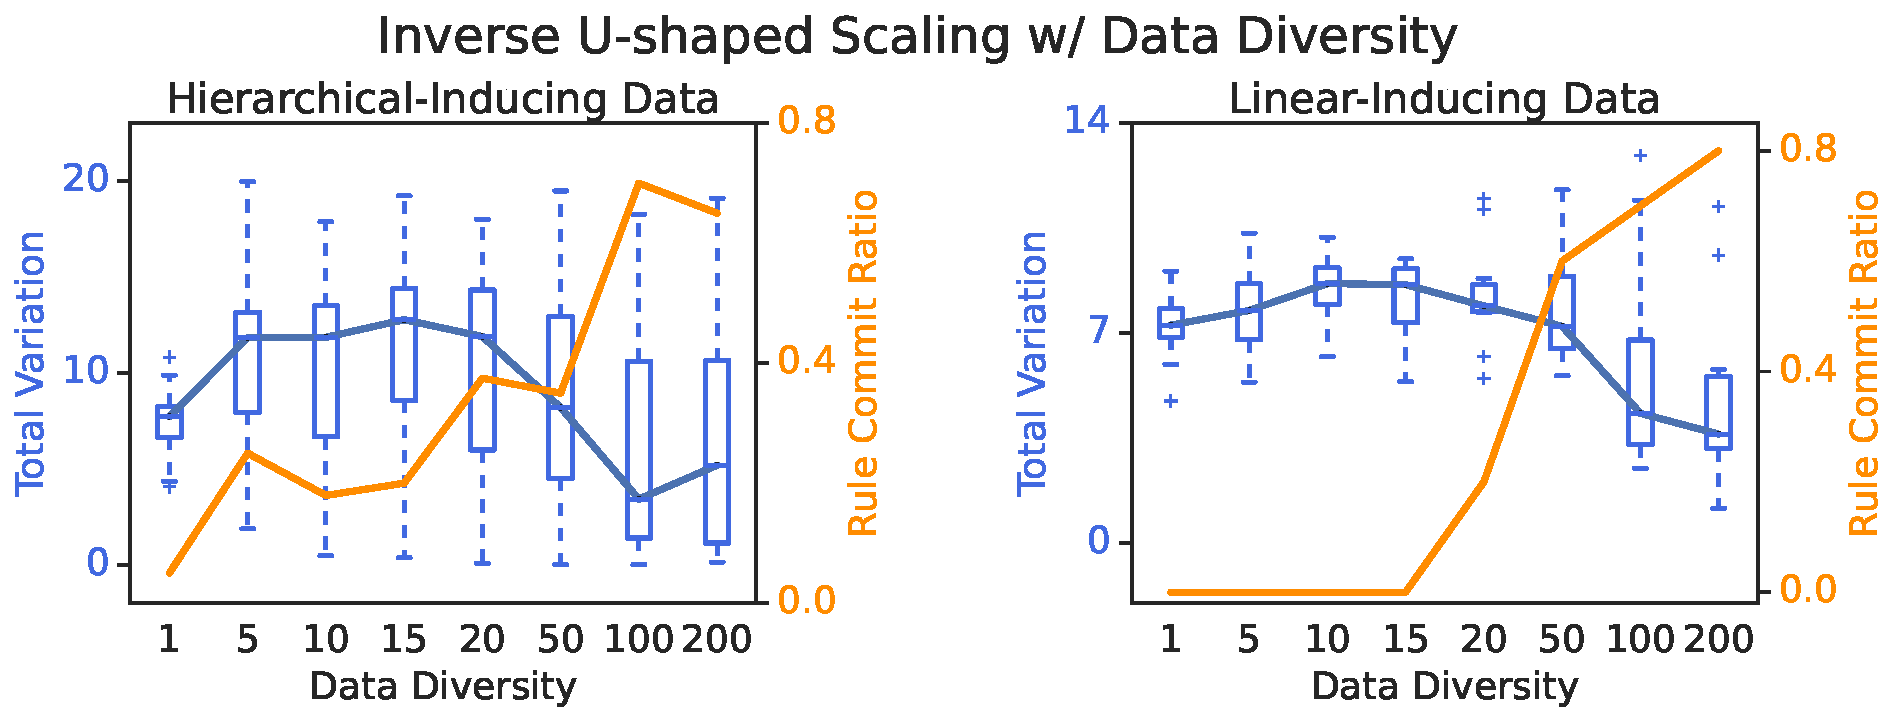
\includegraphics[width=0.8\linewidth]{figures/data_diversity_uscale.pdf}
    \caption{\textbf{Inverse U-shaped relationship between training stability and data diversity.} Whether training data favors the hierarchical (\textit{left}) or linear (\textit{right}) rule, diverse data promotes systematic rules over example memorization. At low diversity, training is stable but the model memorizes individual syntactic patterns rather than committing to a rule. With moderate data diversity, training becomes unstable. As diversity increases further, the model commits to a rule and training is the most stable.} 
    \label{fig:data_diversity_uscale}
    \vspace{-4px}
\end{figure}
\newpage
\section{Early investigations on visual quality in more complex environments}
\label{app:additonal_experiments}

In the main body of the paper, we evaluated the utility of \textsc{diamond} for the purpose of training RL agents in a world model on the well-established Atari 100k benchmark \citep{kaiser2019atari100k}, and demonstrated \textsc{diamond}'s diffusion world model could be applied to model a more complex 3D environment from the game \textit{Counter-Strike: Global Offensive}. In this section, we provide early experiments investigating the effectiveness of \textsc{diamond}'s diffusion world model by directly evaluating the visual quality of the trajectories they generate. The two environments we consider are presented in Section \ref{app:subsec:environments} below.

\subsection{Environments}
\label{app:subsec:environments}

\textbf{CS:GO.} 
We use the \textit{Counter-Strike: Global Offensive} dataset introduced by \citet{pearce2022counter}. Here we use the \textit{Clean} dataset containing 190k frames (3.3 hours) of high-skill human gameplay, captured on the \textit{Dust II} map. This contains observations and actions (mouse and keyboard) captured at 16Hz. We use 150k frames (2.6 hours) for training and 40k frames (0.7 hours) for evaluation. We resize observations to 64$\times$64 pixels, and use no augmentation.
%\footnote{\href{https://github.com/TeaPearce/Counter-Strike_Behavioural_Cloning}{\texttt{https://github.com/TeaPearce/Counter\-Strike\_Behavioural\_Cloning}}}.

\textbf{Motorway driving.} We use the dataset from \citet{santana2016learning}\footnote{\href{https://github.com/commaai/research}{\texttt{https://github.com/commaai/research}}}, which contains camera and metadata captured from human drivers on US motorways. We select only trajectories captured in daylight, and exclude the first and last 5 minutes of each trajectory (typically traveling to/from a motorway), leaving 4.4 hours of data. We use five trajectories for training (3.6 hours) and two for testing (0.8 hours). We downsample the dataset to 10Hz, resize observations to 64$\times$64, and for actions use the (normalized) steering angle and acceleration. During training, we apply data augmentation of shift \& scale, contrast, brightness, and saturation, and mirroring.

We note that the purpose of our investigation is to train and evaluate \textsc{diamond}'s diffusion model on these static datasets, and that we do not perform reinforcement learning, since there is no standard reinforcement learning protocol for these environments.


\subsection{Diffusion Model Architectures}

We consider two potential diffusion model architectures, summarized in Figure \ref{fig_architectures}.

\begin{figure}[h]
    \begin{center}
    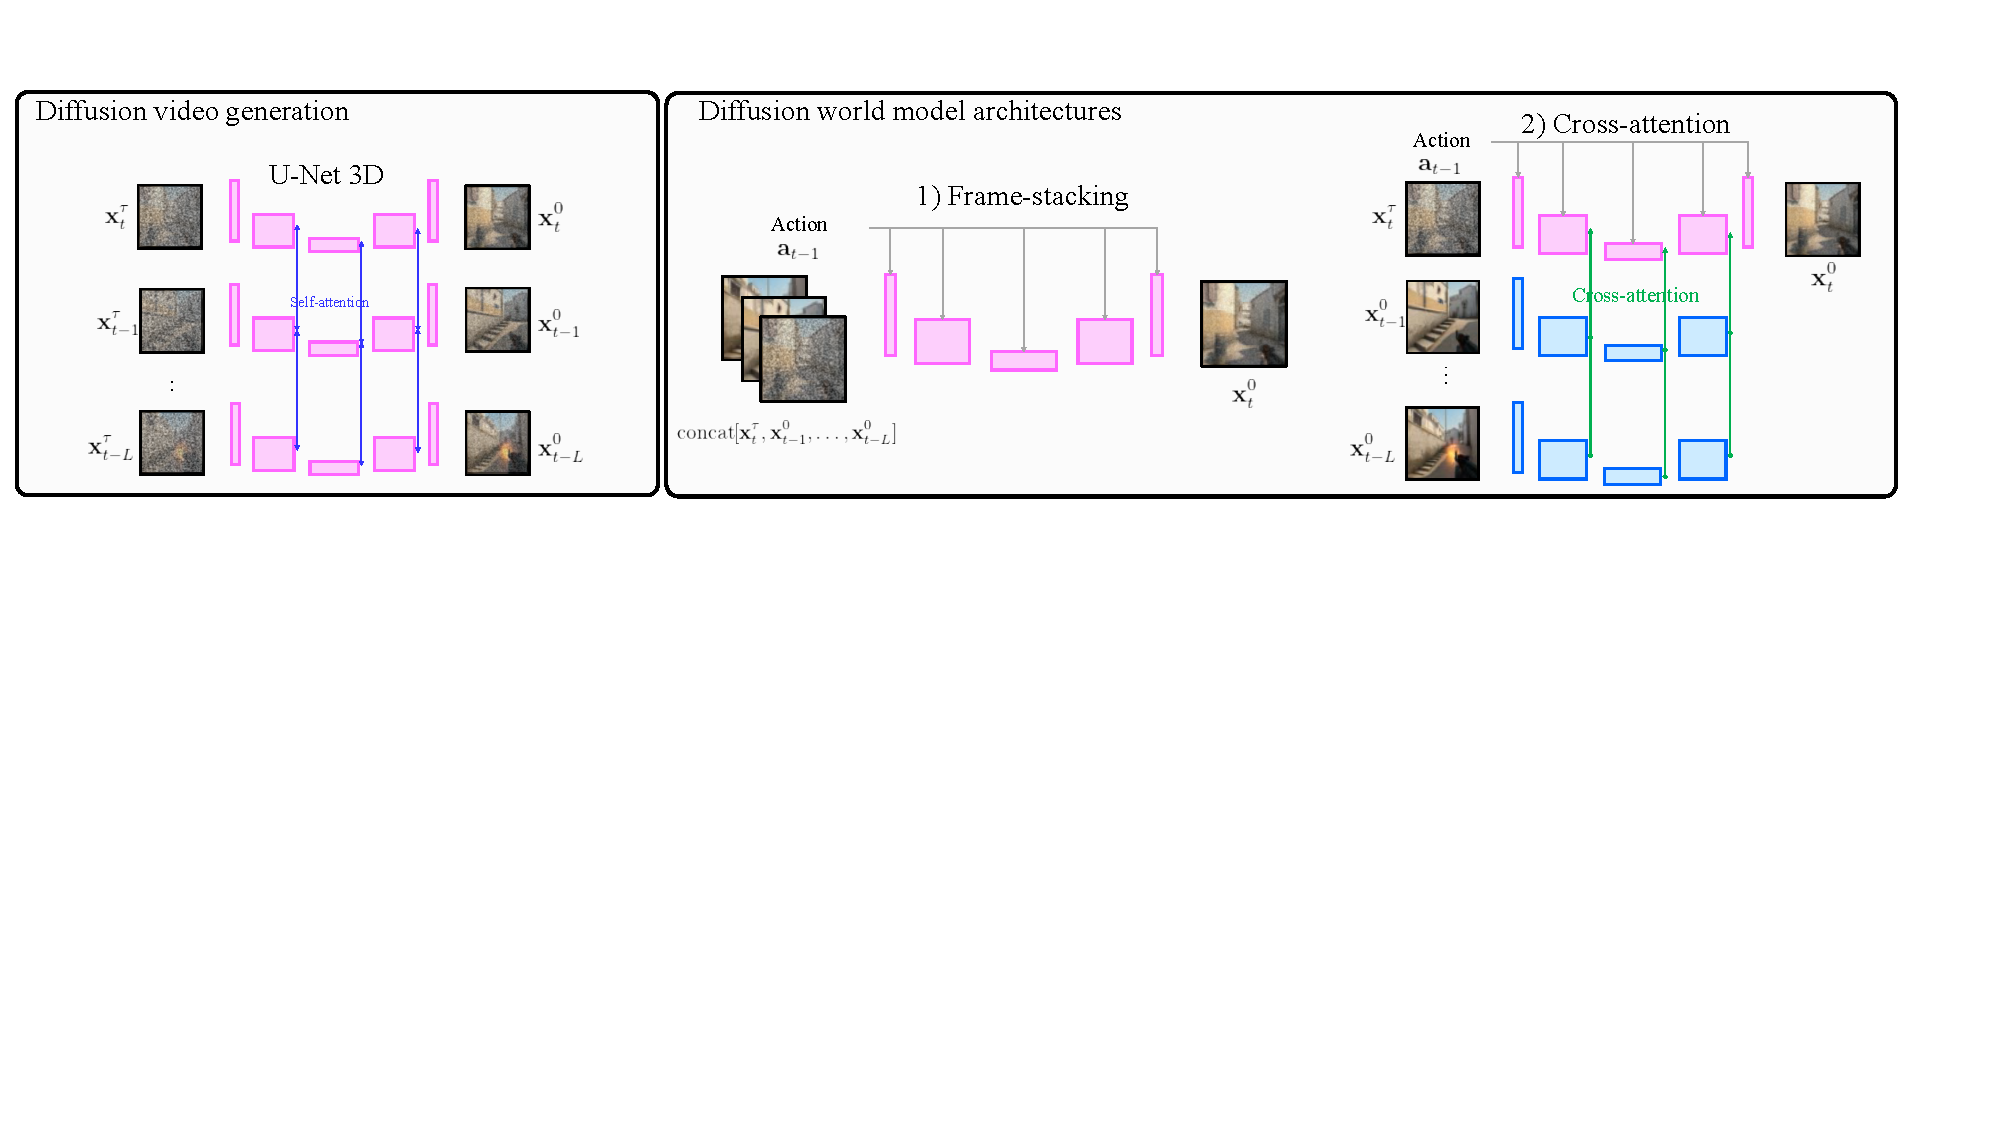
\includegraphics[width=0.99\columnwidth]{images/architectures_02.pdf}
    % \vskip -0.18in
    \caption{We tested two architectures for \textsc{diamond}'s diffusion model which condition on previous image observations in different ways. To illustrate differences with typical video generation models, we also visualize a U-Net 3D \citep{unet3d} which diffuses a block of frames simultaneously.}
    \label{fig_architectures}
    \end{center}
\end{figure}

\textbf{Frame-stacking.} The simplest way to condition on previous observations is by concatenating the previous $L$ frames together with the next noised frame, $\operatorname{concat}[ \x_t^{\tau}, \x_{t-1}^0, \dots, \x_{t-L}^0]$, which is compatible with a standard U-Net 2D \citep{ronneberger2015unet}.
This architecture is particularly attractive due to its lightweight construction, requiring minimal additional parameters and compute compared to typical image diffusion. This is the architecture we used for the main body of the paper.
% Experiments in Section \ref{sec_experiments} show this to be a surprisingly powerful mechanism for modeling both simple and complex environments. 

\textbf{Cross-attention.} 
The U-Net 3D \citep{unet3d}, also displayed for comparison in Figure \ref{fig_architectures}, is a leading architecture in video diffusion \citep{ho2022video}. We adapted this design to have an autoregressive cross-attention architecture, formed of a core U-Net 2D, that only receives a single noised frame as direct input, but which cross-attends to the activations of a separate history encoder network. This encoder is a lightweight version of the U-Net 2D architecture. Parameters are shared for all $L$ encoders, and each receives the relative environment timestep embedding as input.
The final design differs from the U-Net 3D which diffuses all frames jointly, shares parameters across networks, and uses self-, rather than cross-, attention.

\subsection{Metrics, Baselines and Compute}
\textbf{Metrics.}
To evaluate the visual quality of generated trajectories, we use the standard Fréchet Video Distance (\textbf{FVD}) \citep{unterthiner2018towards} as implemented by \citet{skorokhodov2022stylegan}. This is computed between 1024 real videos (taken from the test set), and 1024 generated videos, each 16 frames long (1-2 seconds). Models condition on $L=6$ previous real frames, and the real action sequence. On this same data, we also report the Fréchet Inception Distance (\textbf{FID}) \citep{heusel2017gans}, which measures the visual quality of individual observations, ignoring the temporal dimension. For these same sets of videos, we also compute the \textbf{LPIPS} loss \citep{zhang2018lpips} between each \textit{pair} of real/generated observations \citep{yan2023teco}.
\textbf{Sampling rate} describes the number of observations that can be generated, in sequence, by a single Nvidia RTX A6000 GPU, per second.

\textbf{Baselines.}
We compare against two well-established world model methods; DreamerV3 \citep{hafner2023dreamerv3} and \textsc{iris} \citep{iris2023}, adapting the original implementations to train on a static dataset. We ensured baselines used a similar number of parameters to \textsc{diamond}. Two variants of \textsc{iris} are reported; image observations are discretized into $K=16$ tokens (as used in the original work), or into $K=64$ tokens (achieved with one less down/up-sampling layer in the autoencoder, see Appendix E of \citet{iris2023}), which provide the potential for modeling higher-fidelity visuals. 
% The full list of hyperparameters is provided in the Appendix.
% IRIS: 35M for autoencoder, 88M for transformer, seq length 8...


\textbf{Compute.}
All models (baselines and \textsc{diamond}) were trained for 120k updates with a batch size of 64, on up to 4$\times$A6000 GPUs. Each training run took between 1-2 days.

\subsection{Analysis}

\begin{table}[h]
\caption{Results for 3D environments. These metrics compare observations from real trajectories and generated trajectories. The generated trajectories are conditioned on an initial set of $L=6$ observations and a real sequence of actions.}
\label{tab:video_results}
\begin{center}
\resizebox{0.999 \columnwidth}{!}{
\begin{tabular}{ l c c c c c c c c}
\toprule
\multicolumn{1}{c}{}  & \multicolumn{3}{c}{ ------------ \textbf{CS:GO} ------------} & \multicolumn{3}{c}{ ----------- \textbf{Driving} ----------- } & \multicolumn{1}{c}{\bf Sample rate} & \multicolumn{1}{c}{\bf Parameters} \\
\multicolumn{1}{l}{\bf Method}  & \multicolumn{1}{c}{\bf FID $\downarrow$} & \multicolumn{1}{c}{\bf FVD $\downarrow$ } & \multicolumn{1}{c}{\bf LPIPS $\downarrow$ } & \multicolumn{1}{c}{\bf FID $\downarrow$} & \multicolumn{1}{c}{\bf FVD $\downarrow$} & \multicolumn{1}{c}{\bf LPIPS $\downarrow$ }  & \multicolumn{1}{c}{\bf (Hz) $\uparrow$} & \multicolumn{1}{c}{\bf (\#)} \\ 
\hline \\
DreamerV3 & 106.8 & 509.1 & 0.173 & 167.5 & 733.7 & 0.160 & 266.7 & 181M \\
IRIS ($K=16$) & 24.5 & 110.1 & 0.129 & 51.4 & 368.7 & 0.188 & 4.2 & 123M \\
IRIS ($K=64$) & 22.8 & 85.7 & 0.116 & 44.3 & 276.9 & 0.148 & 1.5 & 111M \\
$\textsc{diamond}$ frame-stack (ours) & 9.6 & 34.8 & 0.107 & 16.7 & 80.3 & 0.058 & 7.4 & 122M \\
$\textsc{diamond}$ cross-attention (ours) & 11.6 & 81.4 & 0.125 & 35.2 & 299.9 & 0.119 & 2.5 & 184M \\
\bottomrule
\end{tabular}
}
\end{center}
\end{table}


Table \ref{tab:video_results} reports metrics on the visual quality of generated trajectories, along with sampling rates and number of parameters, for the frame-stack and cross-attention \textsc{diamond} architectures, compared to baseline methods. 
\textsc{diamond} outperforms the baselines across all visual quality metrics. 
This validates the results seen in the wider video generation literature, where diffusion models currently lead, as discussed in Section \ref{sec:related_work}.
The simpler frame-stacking architecture performs better than cross-attention, something surprising given the prevalence of cross-attention in the video generation literature. We believe the inductive bias provided by directly feeding in the input, frame-wise, may be well suited to autoregressive generation. Overall, these results indicate \textsc{diamond} frame-stack $>$ \textsc{diamond} cross-attention $\approx$ IRIS 64 $>$ IRIS 16 $>$ DreamerV3, which we found corresponds to our intuition from visual inspection.

In terms of sampling rate, \textsc{diamond} frame-stack (with 20 denoising steps) is faster than \textsc{iris} ($K=16$). \textsc{iris} suffers from a further 2.8$\times$ slow down for the $K=64$ version, verifying its sample time is bottlenecked by the number of tokens $K$.
On the other hand, DreamerV3 is an order of magnitude faster -- this derives from its independent, rather than joint, sampling procedure, and the flip-side of this is the low visual quality of its trajectories. 

\newpage


Figure \ref{fig_generation_egs} below shows selected examples of the trajectories produced by \textsc{diamond} in CS:GO and motorway driving.
% Trajectories produced by baselines are given in Appendix \tp{x}.
% , and comparisons with baselines in Appendix Figures \tp{x} \& \tp{y}.
The trajectories are plausible, often even at time horizons of reasonable length. In CS:GO, the model accurately generates the correct geometry of the level as it passes through the doorway into a new area of the map. In motorway driving, a car is plausibly imagined overtaking on the left.

\begin{figure}[h!]
    \begin{center}
    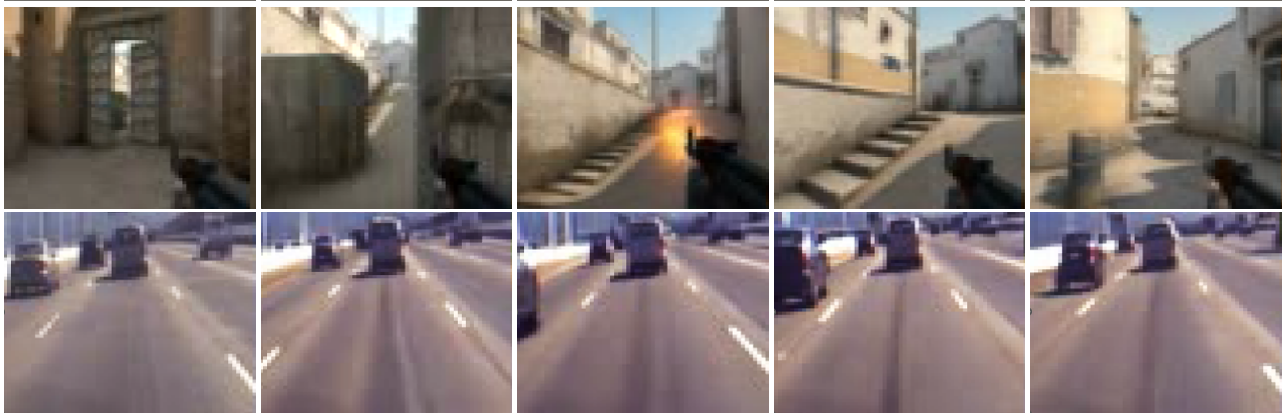
\includegraphics[width=0.8\columnwidth, height=0.4\columnwidth]{images/generation_egs_02.png}
    % \vskip -0.18in
    \caption{Example trajectories sampled every 25 timesteps from \textsc{diamond} (frame stack) for the modern 3D first-person shooter CS:GO (top row), and real-world motorway driving (bottom row).}
    \label{fig_generation_egs}
    \end{center}
\end{figure}


While the above experiments use real sequences of actions from the dataset, we also investigated how robust $\textsc{diamond}$ (frame stack) was to novel, user-input actions.
Figure \ref{fig_driving_action} shows the effect of the actions in motorway driving -- conditioned on the same $L=6$ real frames, we generate trajectories conditioned on five different action sequences. In general the effects are as intended, e.g. steer straight/left/right moves the camera as expected.
Interestingly, when `slow down' is input, the distance to the car in front decreases since the model predicts that the traffic ahead has come to a standstill.
%This is an interesting causal confusion, since from the action alone, slowing down should in principle \textit{increase} the distance to the car in front. 
Figure \ref{fig_csgo_action} shows similar sequences for CS:GO. For the common actions (mouse movements and fire), the effects are as expected, though they are unstable beyond a few frames, since such a sequence of actions is unlikely to have been seen in the demonstration dataset.
% We found that $\textsc{wm}$ had not learned to model the impact of less common actions such as `jump'.
We note that these issues -- the causal confusion and instabilities -- are a symptom of training world models on offline data, rather than being an inherent weakness of $\textsc{diamond}$.
% Also acknowledge the offdistribution problem, but more a problem of data than model.


\begin{figure}[h!]
    \begin{center}
    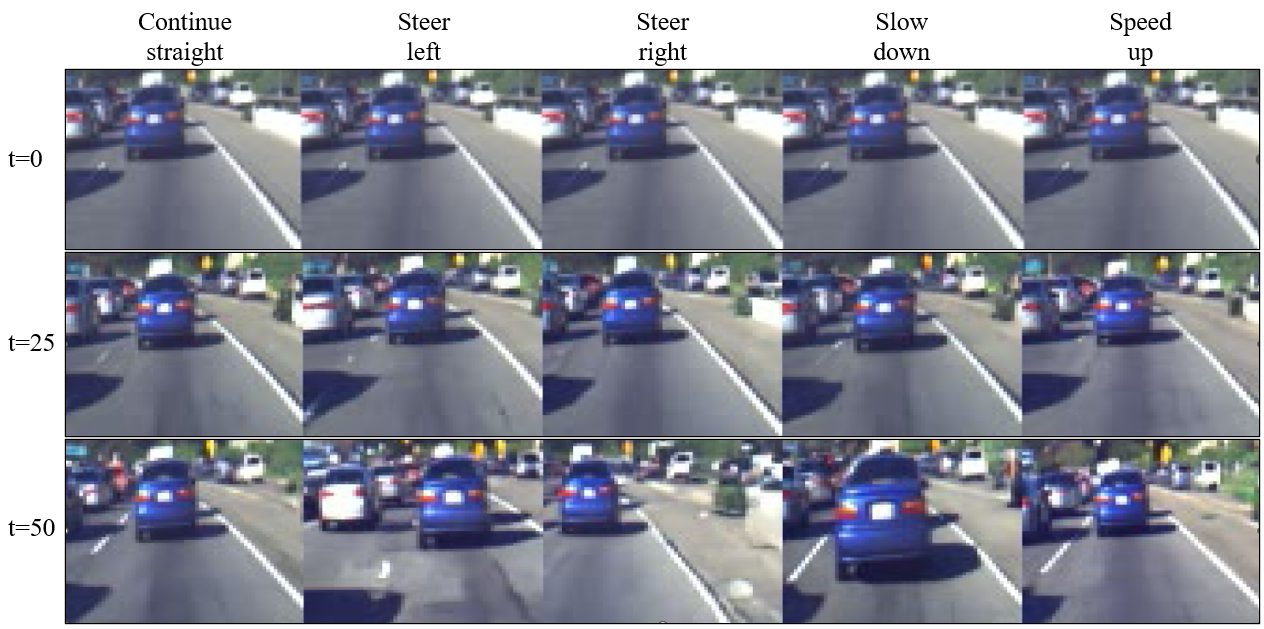
\includegraphics[width=0.99\columnwidth]{images/driving_action_02.png}
    % \vskip -0.18in
    \caption{Effect of fixed actions on sampled trajectories in motorway driving. Conditioned on the same initial observations, we rollout the model applying differing actions. Interestingly, the model has learnt to associate 'Slow down' and 'Speed up' actions to the whole traffic slowing down and speeding up.}
    \label{fig_driving_action}
    \end{center}
\end{figure}


\begin{figure}[t!]
    \begin{center}
    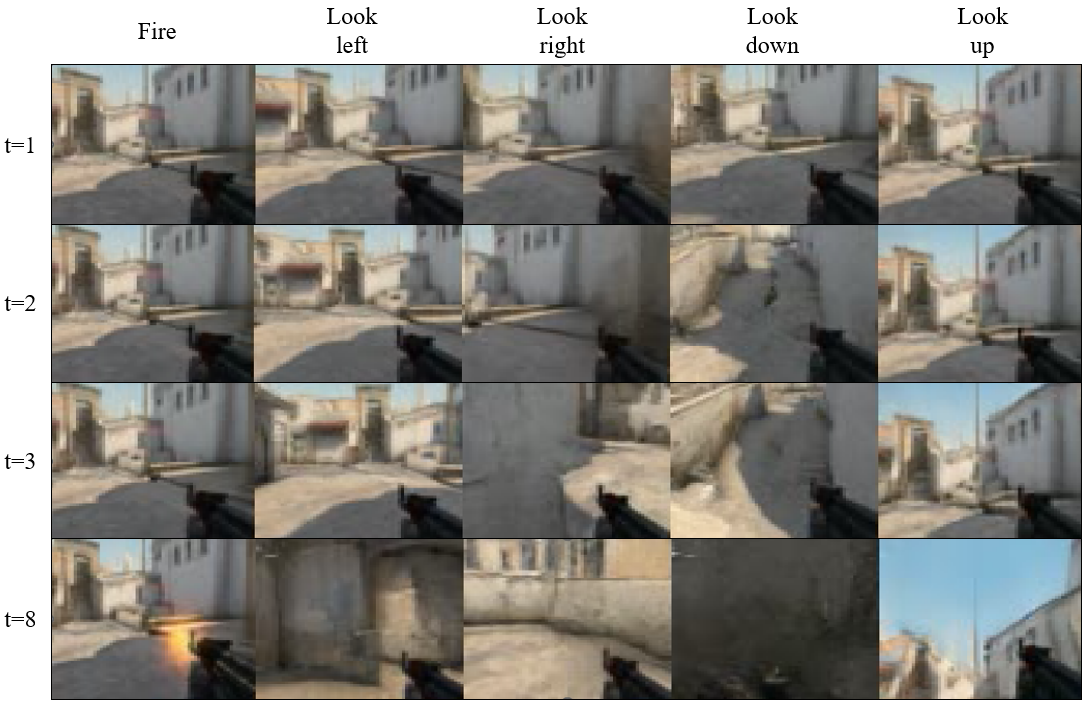
\includegraphics[width=0.9\columnwidth]{images/csgo_action_01.png}
    % \vskip -0.18in
    \caption{Effect of fixed actions on sampled trajectories in CS:GO. Conditioned on the same initial observation, we rollout the model applying differing actions. Whilst in immediate frames these have the intended effect, for longer roll-outs the observations can degenerate. For instance, it would have been very unlikely for the human demonstrator to look directly into ground in this game state, so the world model is unable to generate a plausible trajectory here, and instead snaps onto another area of the map when looking down does make sense.}
    \label{fig_csgo_action}
    \end{center}
\end{figure}
\clearpage


%%%%%%%%%%%%%%%%%%%%%%%%%%%%%%%%%%%%%%%%%%%%%%%%%%%%%%%%%%%%

\end{document}
